% COGNITIVE GRAPH THEORY - REVISED VERSION
% Author: Zeng Mingjia
% Date: \today

\documentclass[12pt,a4paper]{article}
\usepackage[UTF8]{ctex}
\usepackage{amsmath,amssymb,amsthm}
\usepackage{graphicx}
\usepackage{booktabs}
\usepackage{multirow}
\usepackage{algorithm}  % 算法环境
\usepackage{algpseudocode}  % 替换 algorithmicx，提供更好的伪代码支持
\usepackage{enumitem}
\usepackage{listings}
\usepackage{xcolor}
\usepackage{caption}
\usepackage{subcaption}
\usepackage{longtable}
\usepackage{arydshln}
\usepackage{float}
\usepackage[sort&compress]{natbib}  % 更强大的引用管理，替换原来的 cite 包
\bibliographystyle{plainnat}  % 引用样式，也可以选 apalike, ieeetr, alpha 等
\usepackage{tikz}
\usetikzlibrary{backgrounds,trees,positioning, shapes,shapes.misc,shadows,  arrows.meta,arrows, calc, decorations.pathreplacing,mindmap}
\usepackage{pgfplots}  % 如果使用坐标轴
\pgfplotsset{compat=1.17}
\usepackage{array}  % 增强表格功能
\usepackage{booktabs}  % 三线表
\usepackage{makecell}  % 多行表头
\usepackage{multirow}  % 多行合并
\usepackage[top=2.5cm, bottom=2.5cm, left=2.5cm, right=2.5cm]{geometry}
% 定义常用列类型
\newcolumntype{C}{>{\centering\arraybackslash}p}  % 居中的固定宽度列
\newcolumntype{L}{>{\raggedright\arraybackslash}p}  % 左对齐的固定宽度列
\newcolumntype{R}{>{\raggedleft\arraybackslash}p}  % 右对齐的固定宽度列

% 小型表格样式
\newcommand{\smalltable}{\scriptsize}
% 算法命令定义 - 修正
\renewcommand{\algorithmicrequire}{\textbf{输入:}}
\renewcommand{\algorithmicensure}{\textbf{输出:}}
\renewcommand{\algorithmiccomment}[1]{\{#1\}}



% 代码样式设置
\lstset{
    basicstyle=\ttfamily\small,
    keywordstyle=\color{blue},
    commentstyle=\color{green},
    stringstyle=\color{red},
    numbers=left,
    numberstyle=\tiny\color{gray},
    stepnumber=1,
    numbersep=5pt,
    backgroundcolor=\color{white},
    showspaces=false,
    showstringspaces=false,
    showtabs=false,
    frame=single,
    rulecolor=\color{black},
    tabsize=2,
    captionpos=b,
    breaklines=true,
    breakatwhitespace=false,
    escapeinside={\%*}{*},
}

% 数学命令
\newcommand{\cognitivespace}{\mathcal{C}}
\newcommand{\cognitivegroup}{\mathbb{G}}
\newcommand{\energyoperator}{\mathcal{E}}
\newcommand{\compressionoperator}{\mathcal{C}}
\newcommand{\migrationoperator}{\mathcal{M}}

% hyperref 最后加载
\usepackage{hyperref}

% 标题
\title{认知的几何、代数与动力学：基于能耗最小化原理的统一图论模型}
\author{曾铭佳}
\date{\today}

\begin{document}

\maketitle

\begin{abstract}
本文构建一个\textbf{基于第一性原理的思想实验平台}，通过几何、代数和动力学三个维度为认知过程提供统一的形式化模型。系统建立在两个核心公设之上：(1) 认知状态可表征为时空中的动态网络（认知图）；(2) 网络演化受能量动力学支配，其核心优化目标是认知能耗最小化。在此公理化基础上，我们引入群论代数结构，用以描述认知操作的封闭性和可逆性，并推导出“概念压缩”与“第一性原理迁移”是系统为达成能耗优化而自然涌现的宏观行为模式。通过一组代数验证实验，我们展示了认知操作如何构成半群，并初步观察到认知对称性与守恒量之间存在对应关系，为理论的数学基础提供了计算证据。

为观察公理系统的内生解释力，我们在包含51、71、91和111个跨领域概念的四个规模上进行了计算实验。\textbf{需要强调的是，这些实验并非旨在与现有AI系统进行性能对标，而是在一个可控的“计算宇宙”中，对比两种认知范式的内在演化逻辑}：代表外部干预设计的“预设算法模型”与仅由两个核心公设驱动的“自然涌现模型”。结果显示，自然涌现模型在四个规模下分别实现了86.9\%、72.3\%、61.4\%和47.9\%的能耗降低。核心发现：系统在不同概念规模下均展现出与人类认知高度一致的组织原则——概念压缩形成稳定的知识结构，原理迁移实现跨领域创造性连接，且系统能够根据认知负荷自适应调整探索-利用策略。这些发现为能量最小化作为认知组织基本原则提供了计算证据。

本工作旨在为理解智能的本质提供一个新的数学视角和理论框架，而非构建可直接应用的工程系统。该框架不仅统一解释了一系列分散的认知现象，更对当前基于统计关联的人工智能范式构成了根本性质疑，指明了通向更具洞察力与能效的智能系统的设计路径。

\textbf{关键词：} 认知图论，能量最小化，群论代数，概念压缩，第一性原理迁移，认知动力学，思想实验

\end{abstract}

\newpage
% ========== SECTION 1: 引言 ==========
\section{引言}

构建一个能够同时描述知识表征、学习动态与创造性思维的计算理论，是认知科学与人工智能领域的核心挑战。现有工作，如语义网络与知识图谱，精于描述知识的静态结构，却拙于刻画其动态演化过程与内在的优化目标。当前人工智能系统，特别是大型语言模型，虽然在特定任务上表现出色，但其运作机制本质上是基于统计关联的暴力计算，缺乏对认知过程的深刻理解。这种“知其然不知其所以然”的现状，限制了AI系统在创造性思维、跨领域迁移和能量效率方面的表现。

本文采取一条与主流研究截然不同的路径。我们并非要构建一个能与人类行为数据精确拟合的工程模型，也无意与现有AI系统进行性能对标。相反，我们的目标是建立一个\textbf{基于第一性原理的思想实验平台}。在这个由少数简洁公理（认知时空与能量动力学）定义的、完全可控的计算宇宙中，我们试图观察和验证认知组织的基本原则如何从微观互动中自发产生。近期，Bowers等人 \cite{bowers2023importance} 对深度学习模型与人类认知的对比研究提出了深刻的方法论批评，指出缺乏严格测试正在阻碍科学进展。本文从一个不同的角度回应这一问题：不是通过改进实证检验的方法，而是通过从第一性原理出发构建一个可计算的思想实验平台，探索认知组织的基本原则。在这个意义上，本文是对Bowers等人呼吁的一种正面建设性回应。

受物理学中“最小作用量原理”和数学中群论的启发，本文提出一个核心论点：认知过程的底层驱动力，是对“认知能耗”这一内部代价的优化，且认知操作具有代数封闭性和结构保持性。基于此，我们构建了一个以“认知时空”与“能量动力学”为第一性原理的公理化系统。为给这个动态系统提供更严格的数学基础，我们进一步引入了群论结构，\textbf{推导}出认知操作在复合下构成半群，并发现认知对称性与守恒量之间存在对应关系。这些代数性质并非人为设定，而是从公理系统中自然延伸出的形式化描述。

本文的主要理论探索包括：
\begin{itemize}
    \item 建立认知图论的完整公理化体系，包含几何、代数和动力学三个维度。
    \item 引入群论结构描述认知操作的代数性质，并通过计算实验验证其可行性。
    \item 提出并对比两种研究范式：代表外部干预的“预设算法设计”与代表自组织的“自然能量涌现”。
    \item 通过严格的计算实验，观察并分析“概念压缩”和“第一性原理迁移”等现象的涌现规律。
\end{itemize}

\textbf{研究范式定位：} 需要特别说明的是，本研究并非旨在构建一个能够精确拟合人类行为数据的认知模型，也不是为了与特定人工智能系统进行性能对标。相反，我们的目标是建立一个\textbf{基于第一性原理的思想实验平台}。Woensdregt等人 \cite{woensdregt2024lessons} 曾指出，在实证证据稀疏或间接的领域，理论发展需要遵循“良性实践”：明确假设、明确备选理论、计算/形式化建模、寻求外部一致性、三角验证。本文的工作可以看作是在认知计算建模领域对这些实践的一次具体应用：我们明确陈述两个公设（实践i），梳理并对比现有理论（实践ii），构建可计算模型进行思想实验（实践iii），寻求与多个认知理论的外部一致性（实践iv），并通过多规模、多类型实验进行三角验证（实践v）。这一方法论立场贯穿全文。

% ========== SECTION 2: 相关工作和理论背景 ==========
\section{相关工作和理论背景}

% ========== SUBSECTION 2.1: 认知计算模型的演进脉络 ==========
\subsection{认知计算模型的演进脉络}

认知计算模型的发展经历了从符号主义到连接主义的范式演进。符号主义模型如ACT-R \cite{anderson2004act} 和SOAR，擅长基于规则的符号处理，但在面对复杂、模糊的真实世界情境时，往往面临组合爆炸问题，其产生式系统难以模拟人类思维的流畅性与灵活性。

连接主义模型，特别是以Transformer架构\cite{vaswani2017attention}和大型语言模型为代表的深度学习\cite{lecun2015deep}，通过神经网络的分布式表征取得了突破性进展。这些模型在感知和模式识别任务上表现优异，但本质上仍是对统计关联的拟合，其运作机制常被视为“黑箱”，难以解释驱动认知结构演化的内在原理。

强化学习\cite{sutton2018reinforcement}等行为主义模型强调了环境交互的重要性，但其试错学习机制往往需要精心设计奖励函数，与人类高效的内在学习机制仍有距离。

总体而言，现有模型大多侧重于描述认知的“什么”（静态结构）或“如何”（行为输出），但较少探讨其“为何”——即驱动认知结构形成与演化的底层目标函数。这为我们从第一性原理出发构建思想实验平台留下了探索空间。

% ========== SUBSECTION 2.1.4: 作为对比基准的预设算法模型 ==========
\subsubsection{作为对比基准的预设算法模型}
\label{subsec:benchmark_model}

为了在思想实验中系统比较不同认知范式的演化逻辑，我们设计了一个模拟传统认知计算范式的基准模型，称为“预设算法模型”。该模型并非当前最优技术的代表，而是一种与“自组织涌现”相对的“外部干预设计”范式，其核心特征如下：
\begin{itemize}
\item \textbf{算法预设}：包含蒙特卡洛优化、显式的概念压缩和原理迁移等主动控制机制。
\item \textbf{知识先验}：基于语义相似度构建初始网络结构。
\item \textbf{控制逻辑}：由认知状态（专注、探索等）驱动操作选择。
\end{itemize}
该模型在后续实验中作为对照基线，用以凸显仅由能量最小化公设驱动的自然涌现模型的独特行为。

\subsubsection{预设算法模型的实现要点}
\label{subsec:preset_implementation}

在计算实现上，预设算法模型对应\texttt{SemanticEnhancedCognitiveGraph}类（见附录代码）。它继承自基础认知图，并集成了以下机制：
\begin{itemize}
    \item \textbf{网络初始化}：基于51/71/91/111个跨领域概念的语义相似度构建初始网络，边权重按公式$E_{ij}=2.0-1.5\cdot\text{sim}(v_i,v_j)$初始化。
    \item \textbf{蒙特卡洛迭代演化}：运行最多10,000次迭代，每次迭代包含认知状态更新、遗忘机制（指数衰减）、根据状态概率选择操作（硬遍历、软遍历、概念压缩、原理迁移），并记录网络平均能耗。
    \item \textbf{操作实现}：硬遍历优先选择低能耗路径，软遍历为随机游走，概念压缩基于邻居数随机压缩并降低能耗，原理迁移尝试通过原理节点寻找更优路径。
    \item \textbf{参数配置}：统一阈值设置见表\ref{tab:multi_scale_config}，与自然涌现模型保持一致。
\end{itemize}
该模型通过显式规则模拟传统认知计算范式，为后续对比提供参照。

% ========== SUBSECTION 2.2: 能量优化视角的启发 ==========
\subsection{能量优化视角的启发}

Karl Friston的自由能原理\cite{friston2010free}为理解大脑功能提供了一个统一的能量优化框架，认为大脑通过最小化预测误差来维持内稳态。这一思想启发了我们将能量优化作为认知过程的第一性原理。本文在此基础上进一步推进：将自由能原理从神经层面的普遍原理具体化为认知层面可操作的动力学，并着重探讨其如何驱动概念压缩、原理迁移等高阶认知现象的形成。

Tenenbaum的概念生长理论\cite{tenenbaum2011grow}从贝叶斯角度描述了概念学习，Gärdenfors的概念空间理论\cite{gardenfors2004conceptual}从几何视角刻画了概念表征。这些工作为理解认知结构提供了宝贵工具：Tenenbaum的概念生长理论从贝叶斯角度描述了概念学习，Gärdenfors的概念空间理论从几何视角刻画了概念表征。然而，它们主要关注静态结构或概率推理，对驱动认知结构演化的能量动力学机制着墨不多。本文试图在此基础上，引入能耗最小化作为动态演化的核心动力。本文试图在这些工作的基础上，引入能量最小化作为动态演化的核心动力。

本文试图在这些工作的基础上，引入能量最小化作为动态演化的核心动力。需要说明的是，这里的“认知能耗”是对自由能原理的一种概念性类比，而非其数学形式的直接应用——我们更关注能耗最小化如何驱动概念压缩与原理迁移的涌现，而非预测误差的变分推理。

% ========== SUBSECTION 2.3: 代数与几何方法的认知建模应用 ==========
\subsection{代数与几何方法的认知建模应用}

代数方法，特别是群论\cite{rotman1995theory}，在认知科学中已有初步探索。Shepard的心理旋转实验暗示心理操作可能具有连续的群结构，但这些研究多停留在现象描述层面。Gärdenfors的概念空间理论提供了优雅的几何描述，但缺乏对认知操作代数结构的系统整合。

本文的一个核心尝试是将群论等代数工具引入认知动力学，为认知操作提供封闭性、可逆性等数学描述。通过构建认知操作半群、认知对称群等概念，我们试图为认知过程的组合与变换建立形式化基础。

\subsubsection{代数结构的代码实现}

为验证代数框架的可计算性，我们在代码中实现了相关结构（具体见附录）：
\begin{enumerate}
\item \textbf{认知操作半群}：将遍历、学习、遗忘、压缩、迁移等操作形式化为半群元素，观察到了操作的复合与结合律。
\item \textbf{认知对称群与守恒量}：实现了概念同构群的检测，并初步观察了对称变换对应的守恒量趋势。
\item \textbf{群作用与轨道}：实现了对称群在认知状态空间上的作用，验证了轨道-稳定子定理的适用性。
\item \textbf{李群描述}：将连续时间认知演化描述为李群上的运动，为分析认知过程的平滑性提供数学工具（离散近似实现）。
\end{enumerate}
注：由于计算复杂性，部分结构（如连续李群）采用离散近似，但理论框架保持完整。

值得一提的是，Glazebrook与Wallace \cite{glazebrook2009small} 也曾将代数工具引入认知网络研究，他们使用群胚（groupoids）描述全球工作空间理论中的对称性与轨道等价关系，并关注测地线形成与相变的几何表示。这一工作与本文共享“认知网络可用代数几何工具研究”的洞见。区别在于：他们的驱动力来自信息论与统计物理的Onsager关系，关注串扰与巨成分的涌现；而本文的驱动力来自能耗最小化公设，关注概念压缩与原理迁移现象。两种框架可视为代数工具在不同理论假设下的平行探索。

% ========== SUBSECTION 2.4: 复杂系统视角下的认知涌现 ==========
\subsection{复杂系统视角下的认知涌现}

复杂系统理论指出，宏观的秩序模式可以从微观元素的简单相互作用中自发产生。这一视角为理解创造性思维等高阶认知功能提供了新思路。然而，现有研究多停留在定性描述层面，缺乏基于第一性原理的可计算涌现模型。

本文的涌现模型正是对这一思路的回应：仅从“认知时空”和“能量动力学”两个简单公设出发，通过计算实验观察“概念压缩”和“第一性原理迁移”等复杂认知现象的自然产生。这使我们能够在可控环境下探讨认知涌现的基本规律。

% ========== SUBSECTION 2.5: 研究启发与本工作的理论定位 ==========
\subsection{研究启发与本工作的理论定位}
\label{subsec:research_gaps_positioning}

综合现有研究脉络，可以看到一些有待深入探讨的方向：

\begin{itemize}
\item \textbf{整合性}：如何将认知的几何结构、代数操作和动力学演化纳入一个统一的形式框架？
\item \textbf{原理性}：能否从少数基本假设出发，推导出认知组织的核心规律，而非仅描述现象？
\item \textbf{机制性}：能量优化在认知过程中的具体作用机制是怎样的？它与创造性思维有何关联？
\item \textbf{涌现性}：复杂认知现象如何从简单规则中自发涌现？能否通过计算实验观察这一过程？
\end{itemize}

本工作旨在围绕这些问题展开探索，尝试建立一个以能量最小化为第一性原理的认知计算框架。具体来说，我们从以下角度进行尝试：

\begin{enumerate}
\item \textbf{整合几何、代数与动力学}：通过动态网络描述认知的几何结构（第3节），引入群论刻画操作的代数性质（第4节），并基于能量动力学驱动系统演化（第5节）。
\item \textbf{从公设推导认知现象}：从两个核心公设（认知时空与能量动力学）出发，探讨“概念压缩”和“第一性原理迁移”等宏观行为如何作为能耗优化的结果自然出现。
\item \textbf{机制探索}：通过计算实验观察能量优化如何塑造认知结构，并分析其与创造性思维的潜在联系。
\item \textbf{涌现观察}：通过对比预设算法模型与自然涌现模型，观察复杂认知行为从简单规则中产生的过程。
\end{enumerate}

\textbf{理论定位}：与现有研究相比，本文工作的独特之处在于：
\begin{itemize}
\item \textbf{核心论点}：认知的底层驱动力是对“认知能耗”这一内部代价的优化，而非外部奖励或信息最大化。
\item \textbf{公理化路径}：从简单公设出发，构建包含几何、代数、动力学的数学框架，并观察其衍生现象。
\item \textbf{可计算的思想实验}：不仅定性描述，更通过计算实验在可控环境中观察理论预测的行为模式。
\end{itemize}

因此，本工作并非要取代现有理论，而是提供一个可供观察和思考的“认知宇宙”，为理解知识内化到灵感涌现的认知谱系提供新的视角。

% ========== SUBSECTION 2.6: 理论背景示意图 ==========
\subsection{理论背景示意图}
\label{subsec:theoretical_background_mindmap}

为直观展示本章所讨论的理论脉络，图\ref{fig:theoretical_background_mindmap}以思维导图形式汇总了相关工作的演进路径、核心概念与本文的理论定位：

\begin{figure}[H]
\centering
\begin{tikzpicture}[
    scale=0.75,
    mindmap,
    every node/.style={concept, execute at begin node=\hskip0pt, align=center, draw, rectangle, rounded corners=3pt, font=\small},
    level 1 concept/.append style={level distance=4.5cm, sibling angle=120, font=\normalsize\bfseries},
    level 2 concept/.append style={level distance=3.5cm, sibling angle=45, font=\small},
    level 3 concept/.append style={level distance=2.5cm, sibling angle=30, font=\footnotesize},
    text=black
]

% 中心主题：认知计算理论
\node[concept, fill=blue!20, text width=2.5cm] {认知计算理论\\脉络与探索}
    [clockwise from=0]
    child[concept color=green!30, grow=30] {
        node[concept, fill=green!20, text width=2.5cm] {符号主义模型\\[2pt]ACT-R, SOAR}
        child[grow=60] {
            node[concept, fill=green!10, text width=2.0cm] {基于规则\\符号处理}
        }
        child[grow=30] {
            node[concept, fill=green!10, text width=2.0cm] {产生式系统\\逻辑推理}
        }
        child[grow=0] {
            node[concept, fill=green!10, text width=2.0cm] {组合爆炸\\灵活性局限}
        }
    }
    child[concept color=orange!30, grow=90] {
        node[concept, fill=orange!20, text width=3cm] {连接主义模型\\[2pt]深度学习, Transformer}
        child[grow=120] {
            node[concept, fill=orange!10, text width=2.0cm] {统计关联\\分布表征}
        }
        child[grow=90] {
            node[concept, fill=orange!10, text width=2.0cm] {大规模预训练\\模式识别}
        }
        child[grow=60] {
            node[concept, fill=orange!10, text width=2.0cm] {可解释性挑战\\缺乏原理}
        }
    }
    child[concept color=purple!30, grow=150] {
        node[concept, fill=purple!20, text width=3cm] {能量优化视角\\[2pt]自由能原理}
        child[grow=180] {
            node[concept, fill=purple!10, text width=2.0cm] {预测误差最小化\\主动推理}
        }
        child[grow=150] {
            node[concept, fill=purple!10, text width=2.0cm] {神经层面原理\\变分贝叶斯}
        }
        child[grow=120] {
            node[concept, fill=purple!10, text width=2.0cm] {认知层面机制\\尚待具体化}
        }
    };

% 第二圈分支
\node[concept, fill=yellow!20, text width=3.0cm] at (330:5) {代数/几何方法\\[2pt]概念空间, 群论}
    [clockwise from=270]
    child[concept color=yellow!30, grow=300] {
        node[concept, fill=yellow!10, text width=2.0cm] {概念空间理论\\几何表征}
    }
    child[concept color=yellow!30, grow=330] {
        node[concept, fill=yellow!10, text width=2.0cm] {群论结构\\认知对称性}
    }
    child[concept color=yellow!30, grow=360] {
        node[concept, fill=yellow!10, text width=2.0cm] {动态演化\\有待整合}
    };

% 第三圈分支
\node[concept, fill=red!20, text width=3.0cm] at (210:5) {复杂系统视角\\[2pt]涌现现象}
    [clockwise from=210]
    child[concept color=red!30, grow=180] {
        node[concept, fill=red!10, text width=2.0cm] {自组织\\临界现象}
    }
    child[concept color=red!30, grow=210] {
        node[concept, fill=red!10, text width=2.0cm] {从简单规则\\产生复杂行为}
    }
    child[concept color=red!30, grow=240] {
        node[concept, fill=red!10, text width=2.0cm] {可计算模型\\有待发展}
    };

% 理论定位（下方中心）
\node[concept, fill=gray!20, text width=4cm] at (0,-5) {\textbf{本文理论定位：思想实验平台}}
    child[concept color=gray!30, grow=-90] {
        node[concept, fill=gray!10, text width=3.0cm, align=center] {
            \textbf{整合几何、代数、动力学}\\
            统一的形式框架
        }
    }
    child[concept color=gray!30, grow=-30] {
        node[concept, fill=gray!10, text width=3.0cm, align=center] {
            \textbf{基于第一性原理}\\
            从公设推演现象
        }
    }
    child[concept color=gray!30, grow=-150] {
        node[concept, fill=gray!10, text width=3.0cm, align=center] {
            \textbf{可计算的涌现观察}\\
            思想实验验证
        }
    };

\end{tikzpicture}
\caption{相关理论背景脉络图：展示了符号主义、连接主义、能量优化、代数/几何方法和复杂系统等主要理论方向的核心观点与待探索之处，以及本文的思想实验定位。}
\label{fig:theoretical_background_mindmap}
\end{figure}

图\ref{fig:theoretical_background_mindmap}以可视化形式呈现了本章的核心内容，突出了现有理论的贡献与开放问题，并点明本文作为思想实验平台的独特定位。

% ========== SECTION 3: 认知图论的公理系统：几何描述 ==========
\section{认知图论的公理系统：几何描述}

本节为认知图论搭建几何层面的公理基础。我们将认知状态视作动态网络，并引入能量动力学作为其演化的第一性原理。从这两个基本公设出发，可以观察到系统呈现出一系列衍生性质，如可迭代性和可回归性。这些性质并非人为设定，而是公设的必然结果，它们为理解认知过程的连续性与稳定性提供了几何视角。

% ========== SUBSECTION 3.1: 基本公设 ==========
\subsection{基本公设}

\textbf{公设一：认知时空（几何表述）}

存在一个认知网络 $G(V,E,t)$，其中：
\begin{itemize}
\item $V = \{v_1, v_2, \ldots, v_n\}$ 是概念节点集合，每个节点 $v_i$ 代表一个基本概念或知识单元。
\item $E \subseteq V \times V$ 是概念关联边集合，每条边 $e_{ij} = (v_i, v_j)$ 代表概念间的语义或功能关联。
\item $t \in \mathbb{R}^+$ 是连续时间参数，网络的拓扑结构 $\Gamma(t)$ 和连接权重 $w_{ij}(t)$ 都随时间演化。
\end{itemize}

这个动态网络构成了认知活动发生的“舞台”，每个认知状态对应网络的一个特定几何配置。网络的几何特性包括：
\begin{itemize}
\item \textbf{度分布} $P(k)$：描述节点的连接性分布。
\item \textbf{聚类系数} $C$：衡量网络的局部聚集程度。
\item \textbf{路径长度} $L$：概念间的最短认知距离。
\item \textbf{模块性} $Q$：网络社区结构的强度。
\end{itemize}

\textbf{公设二：能量动力学（几何表述）}

认知网络的演化受能量动力学支配：

\begin{enumerate}
\item \textbf{认知能耗函数}：对于任意边 $e_{ij} \in E$，存在认知能耗函数：
\begin{equation}
E_{ij}(t) = f(\Delta_{ij}, s_{ij}, h_{ij}(t), \Theta)
\end{equation}
其中：
\begin{itemize}
\item $\Delta_{ij}$ 是节点间的结构差异性（几何距离）。
\item $s_{ij}$ 是语义关联强度。
\item $h_{ij}(t)$ 是遍历历史熟练度。
\item $\Theta$ 是个体认知参数。
\end{itemize}

\item \textbf{能耗演化机制}：边的能耗动态受历史遍历调控：
\begin{equation}
E_{ij}(t+1) = g(E_{ij}(t), H_{ij}(t), \Theta)
\end{equation}
其中 $H_{ij}(t) = \{(t_k, \tau_k)\}$ 是时间 $t$ 之前的遍历历史记录。

\item \textbf{优化方向}：系统长期演化趋向于最小化全局认知自由能：
\begin{equation}
F(G) = \sum_{e_{ij} \in E} E_{ij} - T \cdot S(G) + R(G)
\end{equation}
其中：
\begin{itemize}
\item $S(G)$ 是网络的结构熵，衡量认知结构的不确定性。
\item $T$ 是认知温度参数，调节探索与利用的平衡。
\item $R(G)$ 是认知资源约束函数。
\end{itemize}
\end{enumerate}

\begin{figure}[H]
\centering
\begin{tikzpicture}[
    scale=1.0,
    every node/.style={circle, draw, minimum size=1.2cm},
    concept/.style={fill=blue!20},
    energy/.style={fill=red!20},
    thick,
    >=stealth
]

% 定义节点位置
\node[concept] (v1) at (-2,1) {算法};
\node[concept] (v2) at (1,2) {递归};
\node[concept] (v3) at (3,1) {神经网络};
\node[concept] (v4) at (0,-2) {模式识别};
\node[concept] (v5) at (4,-2) {优化};
\node[energy] (v6) at (7,-3) {认知能耗};

% 连接边并标注权重
\draw[->] (v1) -- node[midway, above left] {0.85} (v2);
\draw[->] (v1) -- node[midway, above] {0.78} (v3);
\draw[->] (v2) -- node[midway, right] {0.92} (v3);
\draw[->] (v2) -- node[midway, left] {0.67} (v4);
\draw[->] (v3) -- node[midway, right] {0.81} (v5);
\draw[->] (v4) -- node[midway, below] {0.74} (v5);
\draw[->] (v5) -- node[midway, right] {0.63} (v6);
\draw[->] (v1) .. controls (-1,1) and (-1,-1) .. node[midway, left] {0.45} (v4);
\draw[->] (v3) .. controls (5,1) and (5,-1) .. node[midway, right] {0.58} (v5);

% 标注
\node[text width=4cm, align=center, font=\small] at (6,4) {认知图 $G(V,E,t)$ \\ 时间 $t$: 迭代次数};
\node[text width=3cm, align=center, font=\small] at (-1,4) {节点: 概念 \\ 边权重: 认知能耗};

% 能量函数示意
\node[rectangle, draw, rounded corners, fill=yellow!20, minimum width=6cm, minimum height=1.5cm, text width=5.5cm, align=left] at (7,1) {
    \textbf{认知能耗函数:} \\
    $E_{ij}(t) = \alpha(1-\text{sim}_{ij}) + \beta\frac{1}{1+H_{ij}(t)} + \gamma\cdot\text{div}_{ij}$ \\
    $\alpha=0.4,\ \beta=0.4,\ \gamma=0.2$
};

\end{tikzpicture}
\caption{认知图的基本结构：节点表示概念，边表示概念间的关联，边权重表示认知能耗。图中展示了算法、递归、神经网络等概念及其关联，认知能耗函数将能耗分解为语义差异、历史熟练度和结构差异三部分。}
\label{fig:cognitive_graph_structure}
\end{figure}

注：认知图论选择图论作为基础框架，是因为图论能够自然表达概念的语境依赖性——同一节点在不同子图中可扮演不同角色（整体或部分），并且可以通过边的动态变化模拟认知演化。例如，“万有引力定律”在物理学语境中是核心原理节点，而在“苹果落地”的感知语境中则成为该事件的一个背景属性。这种角色转换对应于认知网络在不同语境下的重构，是图论动态性的直接体现。

% ========== SUBSECTION 3.2: 几何衍生性质 ==========
\subsection{几何衍生性质}

下述性质并非独立假设，而是上述公设的必然推论。在思想实验中，我们可以观察到系统在这些公设下自然呈现出的行为模式。

\textbf{性质1：可迭代性（几何表述）}

认知时空 $G(V,E,t)$ 的动态性由其自身的演化方程定义：
\begin{equation}
G(t+1) = \Phi(G(t), I(t), \Theta)
\end{equation}
其中 $\Phi$ 是认知演化算子，$I(t)$ 是外部输入，$\Theta$ 是系统参数。

这个过程将“历史状态”与“新输入”通过认知算法处理，迭代出“新状态”，并依据能量动力学优化网络几何结构。例如，从生疏到熟练的驾驶技能，可以看作 $G(t)$ 在驾驶经验反复迭代下，相关边能耗被持续降低的动力学过程。

\textbf{性质2：可回归性（几何表述）}

系统的任何状态 $G(t)$ 都是其构建历史的完整几何记录。可形式化表示为：
\begin{equation}
G(t) = F(A_1, A_2, \ldots, A_t; G(0))
\end{equation}
其中 $A_i$ 是历史算法操作序列，$G(0)$ 是初始状态。

这意味着系统的当前几何状态是其全部历史的“路径积分”，可回归性正是这一路径依赖特性的外在表现。该性质保证了知识的稳定性，并解释了为何通过复习（重新遍历历史路径）可快速恢复熟练度。例如，故乡记忆在特定气味触发下的瞬间鲜活再现，可以理解为系统回归到历史某一高保真认知状态 $G(t_0)$ 的几何体现。

分析上述两种性质，我们得到，“可迭代性”与“可回归性”均由“时间”带来，或是说“动力学”带来的，其形式化表述为：
原本处在平面上的认知图论，因为时间，使维度由2维平面到3维空间，导致每个节点概念在时间维度上的不断演化，同时这种演化发生理应是需要非本节点概念的外部输入才能有效进行，所以进而出现“可迭代性”；而原本的图理论上是完全图，导致其任意一个节点概念都可以访问另外一个节点概念的关于时间的任意位置，导致出现“可回归性”。

% ========== SUBSECTION 3.3: 数学形式化 ==========
\subsection{数学形式化}
为使理论更具可计算性与可验证性，本节给出核心概念的初步数学形式化描述。这些形式化定义为我们后续在思想实验中观察和测量认知现象提供了基础。

\textbf{认知能耗函数}：为将公设二具体化，我们可以定义边 $e_{ij}$ 在时刻 $t$ 的认知能耗函数如下：
\begin{equation}
E_{ij}(t) = \alpha \cdot (1 - \text{sim}(v_i, v_j)) + \beta \cdot \frac{1}{1 + H_{ij}(t)} + \gamma \cdot \text{div}(v_i, v_j)
\label{eq:energy_function}
\end{equation}
其中：
\begin{itemize}
    \item $\text{sim}(v_i, v_j) \in [0, 1]$ 表示节点 $v_i$ 与 $v_j$ 之间的语义或结构相似度。
    \item $H_{ij}(t)$ 表示到时刻 $t$ 为止，边 $e_{ij}$ 被成功遍历的总次数（历史熟练度）。
    \item $\text{div}(v_i, v_j)$ 表示节点 $v_i$ 与 $v_j$ 在认知网络中的结构差异性（如特征向量的余弦距离）。
    \item $\alpha, \beta, \gamma$ 为权重参数，满足 $\alpha + \beta + \gamma = 1$，用于调节不同因素对总能耗的贡献比例。
\end{itemize}

\textbf{概念压缩的触发条件}：节点集合 $C = \{v_1, v_2, \ldots, v_k\}$ 可被压缩为一个宏观节点 $v_C$，当且仅当满足以下条件：
\begin{equation}
\frac{1}{|C|}\sum_{v_i \in C} \overline{E_{i, \text{external}}} > \theta_c \cdot (E_{C, \text{internal}} + \overline{E_{C, \text{external}}})
\label{eq:compression_condition}
\end{equation}
其中：
\begin{itemize}
    \item $\overline{E_{i, \text{external}}}$ 是集群 $C$ 内节点 $v_i$ 与集群外节点连接的平均能耗。
    \item $E_{C, \text{internal}}$ 是压缩后，宏观节点 $v_C$ 维持其内部结构的能耗（通常极低）。
    \item $\overline{E_{C, \text{external}}}$ 是压缩后，宏观节点 $v_C$ 与外部关键节点连接的平均能耗。
    \item $\theta_c > 1$ 是压缩触发阈值。此不等式的含义是：当维持原有分散结构的平均外部能耗，高于维持压缩后新结构的总能耗某一阈值时，压缩成为能量上的最优解。
\end{itemize}

% ========== SUBSECTION 3.4: 认知遍历的几何理论 ==========
\subsection{认知遍历的几何理论}

作为能量动力学的操作实现，系统演化依赖于两种基本的认知遍历模式。这两种模式在几何上对应着在认知空间中的不同运动方式。

\textbf{定义3.4.1（硬遍历）}：指系统沿着已有的低能耗路径进行精确、高效的思维操作，其特征是路径确定性高、认知能耗相对较低但精度要求高，主要服务于知识的巩固和应用。几何上表现为在认知空间的已知低维流形上运动。

\textbf{定义3.4.2（软遍历）}：指系统以较高的探索性代价搜索新的或弱关联路径，其特征是路径随机性强、认知能耗较高但容忍不确定性，主要服务于知识的探索和创新。几何上表现为在认知空间的高维或未知区域探索。

粗俗点来说，硬遍历像高处向下流的水，方向明确；软遍历像倒在平面上的水，从中心向外扩撒。

% ========== SUBSECTION 3.5: 全文语境假设 ==========
\subsection{全文语境假设}

本研究的理论框架与实验设计基于一个明确的前提假设：所有认知活动发生在\textbf{单一静态语境}之中。所谓单一静态语境，是指在同一认知场景下，概念节点及其关联边所构成的网络结构不因语境切换而改变，整个演化过程均在一个固定的“认知舞台”上展开。这类似于物理学中研究理想气体时所采用的“孤立系统”假设——虽然现实气体总会与外界交换能量，但孤立系统的简化使我们能首先揭示压强、温度等核心变量的基本规律。

\subsubsection{为何需要此假设}

现实中的认知过程总是高度语境依赖的：同一个知识单元（如“万有引力定律”）在物理学课堂上是核心原理，在描述“苹果掉落”的日常事件中则退居背景常识，其语义角色和关联强度会随语境而变化。若在建模之初即引入多语境机制，将同时面临概念表征的动态演化与语境切换的双重复杂性，难以清晰剥离能量最小化原则本身的作用。因此，我们首先在单一静态语境下建立基础模型，专注于观察“认知能耗最小化”这一核心驱动力如何塑造认知结构，待基本规律明晰后再逐步融入语境维度。

\subsubsection{图论框架对语境扩展的天然支持}

尽管当前研究采用静态语境假设，但图论本身为动态语境的建模预留了充分接口：
\begin{itemize}
    \item \textbf{语境节点}：可引入超节点表示特定语境，该节点与语境下活跃的概念节点相连，语境切换时激活不同的子图。
    \item \textbf{动态边权重}：边的认知能耗可设计为受语境参数调制，例如 $E_{ij}(t, c) = f(\Delta_{ij}, s_{ij}, h_{ij}(t), c)$，其中 $c$ 为语境标识。
    \item \textbf{语境演化算子}：认知操作可扩展为包含语境切换的算子，使系统在不同语境间迁移时自动调整网络拓扑。
\end{itemize}
因此，本工作所建立的静态语境模型是迈向动态语境认知模拟的第一步。

\subsubsection{语言文化作为语境差异的例证}

不同语言对同一客观事件的表征方式，可以看作一种天然的语境差异。以“苹果掉落”这一事件为例：
\begin{itemize}
    \item \textbf{英文（还原论倾向）}：“apple falls”可进一步拆分为“apple”（苹果）和“falls”（掉落），每个单词又可分解为词根（如“fall”的基本含义），形成层级化的还原结构。
    \item \textbf{中文（整体论倾向）}：“苹果掉落”可拆分为“苹”、“果”、“掉”、“落”四个单字。每个单字本身蕴含丰富的文化意象和引申含义，例如“苹”从草字头暗示与植物相关，“果”可引申为“结果”、“因果”，“落”则包含“下落”、“衰落”、“村落”等多重意涵。这些单字的不同组合（如“果落”）又能产生新的隐喻（如“结果到来”）。
\end{itemize}
这种差异可能导致中文语义网络比英文语义网络具有更密集的横向关联和更深的历史文化积淀，从而可能影响概念压缩与原理迁移的动力学特征。未来研究可将语言文化作为语境变量，探索不同文化背景下认知图论的普适性与特异性。

总之，本文的静态语境假设是理论发展的必要简化，它为后续引入动态语境、跨文化认知比较等扩展研究奠定了坚实的基础。

% ========== SECTION 4: 认知图论的代数结构：群论描述 ==========
\section{认知图论的代数结构：群论描述}

在前一节中，我们从几何层面将认知状态刻画为动态网络。本节尝试引入代数工具，为认知操作提供更结构化的描述。群论作为研究对称性和变换的数学语言，可以帮助我们理解认知操作之间的组合关系、可逆性以及可能存在的守恒量。需要说明的是，这里提出的代数结构是一种形式化尝试，旨在为后续的认知动力学分析提供一个抽象的数学视角，而不是在断言现实认知必然严格遵循群的所有公理。

% ========== SUBSECTION 4.1: 认知操作的代数系统 ==========
\subsection{认知操作的代数系统}

为了给认知图论提供更丰富的数学描述，我们尝试用代数结构来刻画基本认知操作之间的相互关系。

\textbf{定义4.1.1（认知状态空间）}：设 $\cognitivespace$ 为所有可能认知状态的集合，即：
\begin{equation}
\cognitivespace = \{G(V,E,t) | t \in \mathbb{R}^+\}
\end{equation}

\textbf{定义4.1.2（基本认知操作）}：考虑以下基本认知操作类型：
\begin{itemize}
\item \textbf{遍历操作} $\tau_{path}$：沿特定路径 $path$ 进行认知遍历。
\item \textbf{学习操作} $\lambda_{edge}$：对特定边进行学习，降低其能耗。
\item \textbf{遗忘操作} $\phi_{edge}$：对特定边进行遗忘，增加其能耗。
\item \textbf{压缩操作} $\kappa_{cluster}$：对概念集群进行压缩。
\item \textbf{迁移操作} $\mu_{bridge}$：通过中介节点建立迁移桥梁。
\end{itemize}

\textbf{观察4.1.3（认知操作半群）}：基本认知操作的集合在复合操作下可以构成一个半群结构。

\textbf{说明}：设 $\mathcal{O}$ 为所有基本认知操作的集合。对于任意两个操作 $o_1, o_2 \in \mathcal{O}$，定义复合操作 $o_2 \circ o_1$ 为先执行 $o_1$ 再执行 $o_2$。由于认知操作的执行具有时序性，复合操作满足结合律但不一定满足交换律。因此，$(\mathcal{O}, \circ)$ 可以被看作一个半群。这一观察为认知过程的组合提供了代数描述。

\begin{figure}[H]
\centering
\begin{tikzpicture}[
    scale=0.70,
    operation/.style={rectangle, draw, rounded corners, minimum width=2.2cm, minimum height=1cm, align=center},
    op1/.style={fill=blue!20},
    op2/.style={fill=green!20},
    op3/.style={fill=orange!20},
    result/.style={fill=red!20},
    space/.style={rectangle, draw, rounded corners, fill=gray!10, minimum width=4cm, minimum height=2cm},
    thick,
    >=stealth,
    node distance=1.5cm
]

% 操作节点
\node[operation, op1] (tau) at (0,3) {遍历操作 $\tau$};
\node[operation, op2, right=of tau] (lambda) {学习操作 $\lambda$};
\node[operation, op3, right=of lambda] (phi) {遗忘操作 $\phi$};

% 复合操作
\node[operation, result, below=2cm of lambda] (composite) at (3,0.5) {复合操作 $\phi\circ\lambda\circ\tau$};

% 连接线表示复合过程
\draw[->, thick] (tau.south) .. controls (tau.south west) and (composite.north west) .. 
    node[midway, left, font=\small, yshift=-0.2cm] {结合律: $(\phi\circ\lambda)\circ\tau$} (composite.north west);
\draw[->, thick] (lambda.south) .. controls (lambda.south) and (composite.north) .. 
    node[midway, right, font=\small, yshift=0.1cm] {$=$} (composite.north);
\draw[->, thick] (phi.south) .. controls (phi.south east) and (composite.north east) .. 
    node[midway, right, font=\small, yshift=-0.2cm] {$\phi\circ(\lambda\circ\tau)$} (composite.north east);

% 单位元
\node[operation, fill=yellow!20, left=of tau] (id) {恒等操作 $id$};
\draw[<->, dashed, thick] (id) -- node[midway, above, font=\small] {单位元} (tau);

% 群作用示意
\node[space] (space) at (9, -3.5) {};
\node[circle, draw, fill=white] (state1) at (8.5, -4) {$G_1$};
\node[circle, draw, fill=white] (state2) at (9.5, -4) {$G_2$};
\node[circle, draw, fill=white] (state3) at (9, -3) {$G_3$};

\draw[->, thick, blue] (composite.east) -- (space.west) 
    node[midway, above, font=\small] {群作用 $\alpha$};
\draw[->, thick, green] (state1) -- node[midway, above, font=\scriptsize] {$\tau$} (state2);
\draw[->, thick, orange] (state2) -- node[midway, right, font=\scriptsize] {$\lambda$} (state3);

% 标注
\node[text width=4cm, align=center, font=\small] at (-7, -3.5) {
    \textbf{认知操作半群 $(\mathcal{O},\circ)$} \\
    $\bullet$ 封闭性: $o_1\circ o_2 \in \mathcal{O}$ \\
    $\bullet$ 结合律: $(o_1\circ o_2)\circ o_3 = o_1\circ(o_2\circ o_3)$ \\
    $\bullet$ 单位元: $id\circ o = o\circ id = o$ \\
    $\bullet$ 不一定有逆元
};

% 添加解释性标签
\node[below=0.5cm of space, font=\small] {认知状态空间 $\mathcal{C}$};

\end{tikzpicture}
\caption{认知操作的代数结构：基本认知操作可以构成一个半群，满足封闭性和结合律。图中展示了遍历$\tau$、学习$\lambda$和遗忘$\phi$三个操作的复合过程，以及它们通过群作用$\alpha$对认知状态空间$\mathcal{C}$的影响。这种代数描述为理解认知过程的组合性质提供了一个形式化视角。}
\label{fig:cognitive_semigroup}
\end{figure}

% ========== SUBSECTION 4.2: 认知对称性与不变性 ==========
\subsection{认知对称性与不变性}

在认知网络中，某些变换可能保持系统的关键性质不变，这种不变性可以用对称群的概念来描述。

\textbf{定义4.2.1（认知对称群）}：设 $\cognitivegroup$ 是保持认知网络某些性质不变的变换群，可以称为认知对称群。

认知对称群可能包含以下子群：
\begin{itemize}
\item \textbf{概念同构群} $Aut(V)$：保持概念语义结构不变的置换群。
\item \textbf{结构同伦群} $\pi_1(\cognitivespace)$：认知空间拓扑结构的刻画。
\item \textbf{能量守恒群} $Iso(E)$：保持全局能量不变的等距变换群。
\end{itemize}

\textbf{观察4.2.2（Noether型对应）}：在物理系统中，连续对称性往往对应守恒量。在认知系统中，我们也可以尝试寻找类似的对应关系。

\textbf{实验观察}：在后续的代数验证实验中，我们观察到：
\begin{itemize}
\item 时间平移对称性与认知能量守恒趋势之间存在关联。
\item 概念置换对称性与结构熵的相对稳定性有一定对应。
\item 尺度变换对称性与分形维数的保持存在趋势。
\end{itemize}

注：这种对应关系在实验中通过对称性检测算法进行了初步观察，但由于认知系统的复杂性，它更多是作为一种启发性的理论视角，而非严格的数学定理。

% ========== SUBSECTION 4.3: 认知操作的群作用 ==========
\subsection{认知操作的群作用}

对称群可以在认知状态空间上发挥作用，这种作用可以用群作用的概念来描述。

\textbf{定义4.3.1（群作用）}：认知对称群 $\cognitivegroup$ 在认知状态空间 $\cognitivespace$ 上可以定义一个群作用：
\begin{equation}
\alpha: \cognitivegroup \times \cognitivespace \rightarrow \cognitivespace
\end{equation}
满足：
\begin{enumerate}
\item $\alpha(e, G) = G$（单位元作用不变）
\item $\alpha(g, \alpha(h, G)) = \alpha(gh, G)$（兼容群乘法）
\end{enumerate}

\textbf{定义4.3.2（轨道与稳定子）}：
\begin{itemize}
\item 状态 $G$ 的轨道：$O_G = \{\alpha(g, G) | g \in \cognitivegroup\}$
\item 状态 $G$ 的稳定子：$Stab(G) = \{g \in \cognitivegroup | \alpha(g, G) = G\}$
\end{itemize}

\textbf{观察4.3.3（轨道-稳定子关系）}：对于有限群作用，轨道大小与稳定子大小之间满足：
\begin{equation}
|O_G| = \frac{|\cognitivegroup|}{|Stab(G)|}
\end{equation}

在认知图论中，这一关系可以帮助我们理解从一个认知状态通过对称变换能够到达的其他状态的数量，从而反映认知系统的可能变化范围。当然，在实际认知网络中，由于个体差异和历史依赖，对称性往往较低，轨道通常很小甚至只有自身。

% ========== SUBSECTION 4.4: 认知演化的李群描述 ==========
\subsection{认知演化的李群描述}

对于连续时间演化，我们可以尝试用李群的语言来描述认知动力学。这为分析认知过程的平滑性和连续性提供了一个理论视角。

\textbf{定义4.4.1（认知演化李群）}：设 $\cognitivegroup$ 是一个李群，其李代数 $\mathfrak{g}$ 的生成元可以对应基本认知操作：

\begin{equation}
\mathfrak{g} = span\{\energyoperator, \compressionoperator, \migrationoperator, \ldots\}
\end{equation}

其中：
\begin{itemize}
\item $\energyoperator$：能量优化算子
\item $\compressionoperator$：概念压缩算子  
\item $\migrationoperator$：原理迁移算子
\end{itemize}

\textbf{观察4.4.2（认知动力学方程）}：认知状态的演化可以用李群上的方程来描述：
\begin{equation}
\frac{dG(t)}{dt} = A(t)G(t), \quad A(t) \in \mathfrak{g}
\end{equation}

这个方程将认知动力学表达为在李群上的运动，为分析认知过程的连续变化提供了一个数学框架。在实际代码实现中，我们采用离散近似来模拟这一连续过程。

注：连续李群描述主要作为理论框架提出，用于启发我们对认知过程连续性的思考，实际计算中仍以离散模型为主。

% ========== SUBSECTION 4.5: 代数结构的认知意义 ==========
\subsection{代数结构的认知意义}

从思想实验的角度看，引入代数结构可以帮助我们更清晰地思考认知过程的形式特征：

\begin{itemize}
\item \textbf{封闭性}：认知操作的复合仍然产生认知操作，这提示认知系统具有一定的自包含性。
\item \textbf{结合律}：操作的执行顺序影响结果，但不影响可执行性，这对应思维过程的连贯性。
\item \textbf{单位元}：存在保持认知状态不变的操作，如“暂停思考”或“维持注意力”。
\item \textbf{逆元}：某些认知操作可能可逆（如学习与遗忘），但并非所有操作都有逆，这反映了认知过程的不可逆性。
\end{itemize}

这些代数性质为我们构建可计算的认知模型提供了数学基础，同时也为思考认知系统的结构保持性提供了工具。

% ========== SUBSECTION 4.6: 代数结构的实现与意义 ==========
\subsection{代数结构的实现与意义}
\label{subsec:algebraic_implementation}

本文提出的代数结构不仅具有理论意义，也在代码中得到了具体实现，用于在思想实验中观察这些形式化概念的实际表现。

\textbf{认知操作半群的实现}：
\begin{itemize}
\item 在代码中将遍历、学习、遗忘等操作封装为\texttt{CognitiveOperation}类。
\item 实现了操作的复合与结合律验证（见附录代码列表1）。
\end{itemize}

\textbf{对称性检测}：
\begin{itemize}
\item 实现了概念同构群的简化检测算法。
\item 初步观察了Noether型对应：在某些对称变换下，系统的某些量（如结构熵）表现出相对稳定性。
\end{itemize}

\textbf{实际与理论的对应关系}：
\begin{table}[H]
\centering
\caption{代数结构的理论概念与代码实现对应关系}
\label{tab:algebraic_implementation}
\begin{tabular}{p{3.0cm}p{5.0cm}p{2.2cm}}
\toprule
\textbf{理论概念} & \textbf{代码实现} & \textbf{实现程度} \\
\midrule
认知操作半群 & \texttt{CognitiveSemigroup}类 & 完全实现 \\
对称群 & \texttt{CognitiveSymmetryGroup}类 & 简化实现 \\
李群演化 & 理论框架 & 仅概念验证 \\
\bottomrule
\end{tabular}
\end{table}

注：由于计算复杂性的考虑，部分代数结构（如连续李群）仅作为理论框架提出，实际代码采用了离散近似。这符合思想实验的特点：我们关注的是概念上的启发性，而非严格的数学完备性。

% ========== SECTION 5: 代数实验 ==========
\section{代数实验：理论框架的计算观察}
\label{sec:algebraic_experiments}

为观察认知图论代数框架在思想实验环境中的行为表现，我们设计并执行了五组计算实验。这些实验旨在探索第4节提出的群论结构在模拟系统中的可操作性，包括认知操作半群的性质、Noether型对应的趋势、轨道-稳定子定理的适用性、李群演化框架的可行性以及代数方法的可扩展性。需要强调的是，这些实验的目的并非在“证明”数学定理，而是在我们定义的计算宇宙中观察这些代数结构是否能够被识别和描述。

% ========== SUBSECTION 5.1: 实验设计 ==========
\subsection{实验设计}
\label{subsec:algebraic_experiment_design}

代数验证实验采用分层探索策略，从基础代数性质到复杂群论结构进行系统性观察：

\textbf{实验1：认知操作半群验证}
\begin{itemize}
    \item \textbf{目的}：观察基本认知操作（遍历、学习、遗忘、压缩、迁移）在复合操作下是否表现出半群性质。
    \item \textbf{方法}：随机生成13种认知操作，测试结合律$(a \circ b) \circ c = a \circ (b \circ c)$。
    \item \textbf{预期}：所有操作组合应满足结合律，但交换律不一定成立。
\end{itemize}

\textbf{实验2：Noether型对应观察}
\begin{itemize}
    \item \textbf{目的}：观察认知对称性与守恒量之间是否存在某种对应关系。
    \item \textbf{方法}：在三个不同结构的认知网络（5节点、10节点、15节点）上检测对称性并计算守恒量的变化。
    \item \textbf{指标}：全局认知能量、结构熵、分形维数的相对变化。
\end{itemize}

\textbf{实验3：轨道-稳定子定理适用性观察}
\begin{itemize}
    \item \textbf{目的}：观察轨道-稳定子定理在认知状态空间中的表现。
    \item \textbf{方法}：计算认知对称群大小$|\cognitivegroup|$、稳定子大小$|Stab(G)|$和轨道大小$|O_G|$。
    \item \textbf{验证}：检查是否满足$|O_G| = \frac{|\cognitivegroup|}{|Stab(G)|}$。
\end{itemize}

\textbf{实验4：李群演化框架演示}
\begin{itemize}
    \item \textbf{目的}：展示连续时间认知演化的李群描述在思想实验中的可行性。
    \item \textbf{方法}：采用三种不同的李代数生成元组合（能量优化主导、概念压缩主导、原理迁移主导）。
    \item \textbf{指标}：演化前后的认知能耗变化百分比。
\end{itemize}

\textbf{实验5：代数方法可扩展性测试}
\begin{itemize}
    \item \textbf{目的}：评估代数方法在不同规模网络中的计算效率。
    \item \textbf{方法}：在5到15个节点的网络上测试半群运算和对称性检测时间。
    \item \textbf{规模}：5、8、10、12、15节点网络。
\end{itemize}

% ========== SUBSECTION 5.2: 实验结果与分析 ==========
\subsection{实验结果与分析}
\label{subsec:algebraic_results}

% ========== SUBSUBSECTION 5.2.1: 认知操作半群验证结果 ==========
\subsubsection{认知操作半群验证结果}
\label{subsubsec:semigroup_results}

实验1观察了13种认知操作的结合律性质，所有测试组合均表现出结合律：

\begin{itemize}
    \item \textbf{结合律验证}：所有操作组合均满足$(a \circ b) \circ c = a \circ (b \circ c)$。
    \item \textbf{关键案例}：
    \begin{itemize}
        \item (学习 $\circ$ 遗忘) $\circ$ 遍历 = 学习 $\circ$ (遗忘 $\circ$ 遍历)：验证通过
        \item (压缩 $\circ$ 迁移) $\circ$ 学习 = 压缩 $\circ$ (迁移 $\circ$ 学习)：验证通过
        \item (遍历 $\circ$ 学习) $\circ$ 遗忘 = 遍历 $\circ$ (学习 $\circ$ 遗忘)：验证通过
    \end{itemize}
    \item \textbf{观察}：认知操作集合在复合操作下表现出半群结构，这与第4.1节的代数描述一致。
\end{itemize}

\textbf{思考意义}：这一结果表明，在思想实验环境中，认知操作的组合确实可以形成封闭的代数系统。这为理解思维过程的连贯性和可组合性提供了一个计算视角。

% ========== SUBSUBSECTION 5.2.2: Noether型对应观察结果 ==========
\subsubsection{Noether型对应观察结果}
\label{subsubsec:noether_results}

实验2在三个不同结构的认知网络上观察了Noether型对应的表现：

\begin{table}[H]
\centering
\caption{Noether型对应观察结果}
\label{tab:noether_results}
\begin{tabular}{p{2cm}cccc}
\toprule
\textbf{网络} & \textbf{同构数} & \textbf{能量守恒趋势} & \textbf{结构熵守恒} & \textbf{分形维数趋势保持} \\
\midrule
网络1 & 1 & 是 & 是 & 是 \\
网络2 & 1 & 是 & 是 & 是 \\
网络3 & 1 & 是 & 是 & 是 \\
\bottomrule
\end{tabular}
\end{table}

\textbf{守恒量分析}：
\begin{itemize}
    \item \textbf{全局认知能量}：三个网络均表现出能量守恒趋势，相对变化小于1\%。
    \item \textbf{结构熵}：完全守恒（相对变化为0）。
    \item \textbf{分形维数}：趋势保持，微小变化（相对变化小于0.2\%）。
\end{itemize}

\textbf{同构数为1的观察}：在认知图论的完全图模型中，每个概念节点虽然都与其他节点连接，但由于认知能耗权重的差异性，网络几乎不存在非平凡的自同构。本实验检测到的同构仅为恒等自同构，这恰好反映了认知系统的个体差异性：
\begin{enumerate}
    \item 每个概念在网络中的位置具有唯一性。
    \item 每条连接的认知能耗编码了特定的学习历史。
    \item 认知结构的低对称性体现了知识的个性化和情境依赖性。
\end{enumerate}

这种低对称性特征与人类认知的典型特点相呼应：每个人的知识网络都是独特的，难以通过简单的节点置换来保持认知结构不变。

% ========== SUBSUBSECTION 5.2.3: 轨道-稳定子定理适用性观察 ==========
\subsubsection{轨道-稳定子定理适用性观察}
\label{subsubsec:orbit_stabilizer_results}

实验3观察了轨道-稳定子定理在认知状态空间中的表现：

\begin{itemize}
    \item \textbf{同构群大小}：$|\cognitivegroup| = 1$
    \item \textbf{稳定子大小}：$|Stab(G)| = 1$
    \item \textbf{轨道大小}：$|O_G| = 1$
    \item \textbf{定理适用性}：$1 = \frac{1}{1}$，关系成立
\end{itemize}

\textbf{理论思考}：轨道-稳定子定理在平凡群作用下成立，这验证了认知状态空间的低对称性特征。稳定子仅包含恒等映射，轨道只包含自身，体现了认知系统的个体独特性。

这里的“平凡验证”恰恰从反面印证了认知系统的一个核心特征：由于学习历史和权重差异性的存在，现实中的认知网络几乎不具备完美的数学对称性。这提醒我们，数学上的“理想群作用”与认知的“现实演化”之间存在张力，未来研究需要在保留代数结构描述力的同时，发展能处理低对称性现实网络的近似方法。

% ========== SUBSUBSECTION 5.2.4: 李群演化框架演示结果 ==========
\subsubsection{李群演化框架演示结果}
\label{subsubsec:lie_group_results}

实验4演示了三种不同生成元组合下的连续演化，观察到了李群描述认知演化的可行性：

\begin{table}[H]
\centering
\caption{李群演化策略的能耗变化}
\label{tab:lie_group_results}
\begin{tabular}{p{3cm}cp{3cm}c}
\toprule
\textbf{策略类型} & \textbf{生成元系数} & \textbf{主导操作} & \textbf{能耗变化} \\
\midrule
能量优化主导 & $\{\mathcal{E}:0.7, \mathcal{C}:0.2, \mathcal{M}:0.1\}$ & 能量优化 & -34.7\% \\
概念压缩主导 & $\{\mathcal{E}:0.3, \mathcal{C}:0.6, \mathcal{M}:0.1\}$ & 概念压缩 & -14.7\% \\
原理迁移主导 & $\{\mathcal{E}:0.2, \mathcal{C}:0.2, \mathcal{M}:0.6\}$ & 原理迁移 & -12.4\% \\
\bottomrule
\end{tabular}
\end{table}

\textbf{观察发现}：
\begin{enumerate}
    \item \textbf{能量优化策略最有效}：以能量优化算子$\mathcal{E}$为主的策略实现了最大能耗降低（34.7\%）。
    \item \textbf{概念压缩的中等效果}：强调概念压缩的$\mathcal{C}$算子产生了14.7\%的优化。
    \item \textbf{原理迁移的探索价值}：虽然直接能耗优化较小（12.4\%），但原理迁移为创造性连接提供了基础。
\end{enumerate}

% ========== SUBSUBSECTION 5.2.5: 代数方法可扩展性结果 ==========
\subsubsection{代数方法可扩展性结果}
\label{subsubsec:scalability_results}

实验5测试了代数方法在不同规模网络中的计算效率：

\begin{table}[H]
\centering
\caption{代数方法可扩展性测试结果}
\label{tab:scalability_results}
\begin{tabular}{cccccc}
\toprule
\textbf{网络规模} & \textbf{半群运算时间(s)} & \textbf{对称性检测时间(s)} & \textbf{同构数} & \textbf{检测成功} & \textbf{计算复杂度} \\
\midrule
5节点 & 0.0000 & 0.0060 & 2 & True & $O(n!)$ \\
8节点 & 0.0000 & 0.0620 & 1 & True & $O(n!)$ \\
10节点 & 0.0000 & 0.0260 & 1 & True & $O(n!)$ \\
12节点 & 0.0000 & 0.0450 & 1 & True & $O(n!)$ \\
15节点 & 0.0000 & 0.0072 & 1 & True & $O(n!)$ \\
\bottomrule
\end{tabular}
\end{table}

\textbf{可扩展性分析}：
\begin{itemize}
    \item \textbf{计算效率}：在15节点规模内，所有代数运算时间小于0.1秒，满足实时性要求。
    \item \textbf{同构数趋势}：随着网络规模增大，同构数基本为1（恒等映射），与认知系统的个体差异性一致。
    \item \textbf{复杂度限制}：对称性检测的复杂度为$O(n!)$，限制了大规模应用，但可通过启发式算法优化。
\end{itemize}

\textbf{实践意义}：代数方法在中等规模认知网络（15节点以内）中具有良好的计算可行性，为思想实验中的实时分析和观察提供了数学工具。

% ========== SUBSECTION 5.3: 综合讨论 ==========
\subsection{综合讨论}
\label{subsec:algebraic_discussion}

五组代数验证实验从不同角度观察了认知图论代数框架在思想实验环境中的行为：

\textbf{1. 代数结构的可观察性}：
\begin{itemize}
    \item 认知操作半群的表现与第4.1节的代数描述一致。
    \item Noether型对应的趋势支持了第4.2.2节观察的合理性。
    \item 轨道-稳定子定理的适用性确认了第4.3.3节关系在简化情况下的成立。
    \item 李群演化演示验证了第4.4.2节方程的实践可行性。
\end{itemize}

\textbf{2. 低对称性的认知意义}：
实验中观察到的低对称性（同构数为0或1）并非算法缺陷，而是认知系统本质特征的反映：
\begin{enumerate}
    \item \textbf{个体差异性}：每个人的知识网络都是独特的。
    \item \textbf{历史路径依赖性}：认知能耗权重编码了学习历史。
    \item \textbf{情境特异性}：认知结构高度依赖于具体情境和经验。
\end{enumerate}

\textbf{3. 计算可行性与局限性}：
\begin{itemize}
    \item \textbf{优势}：代数方法为认知过程提供了严格的数学描述和可观察的预测。
    \item \textbf{局限}：对称性检测的阶乘复杂度限制了大规模应用。
    \item \textbf{改进方向}：开发启发式算法和近似方法处理大规模网络。
\end{itemize}

\textbf{4. 与人类认知的对应关系}：
代数验证实验的结果与人类认知的多个特征形成了有趣的对应：
\begin{itemize}
    \item 认知操作的结合律对应思维过程的连贯性和可组合性。
    \item 能量守恒趋势对应认知资源的有限性和优化需求。
    \item 低对称性对应个体认知风格的独特性和不可互换性。
    \item 连续演化对应思维过程的流畅性和渐进性。
\end{itemize}

% ========== SUBSECTION 5.4: 实验小结 ==========
\subsection{实验小结}
\label{subsec:algebraic_conclusion}

通过这组代数验证实验，我们对认知图论代数框架的核心概念有了更直观的认识：

\begin{enumerate}
    \item \textbf{认知操作半群可被观察}：基本认知操作在复合下满足结合律，表现出半群结构。
    \item \textbf{Noether型对应表现出趋势}：认知系统在演化过程中保持核心守恒量的相对稳定。
    \item \textbf{轨道-稳定子定理在简化情况下适用}：在认知状态空间的对称变换下，轨道与稳定子的关系成立。
    \item \textbf{李群演化框架具有可行性}：连续时间认知演化可用李群方程描述，不同策略产生不同的能耗优化效果。
    \item \textbf{代数方法在中等规模可行}：在15节点以内，代数方法的计算效率满足思想实验需求。
\end{enumerate}

这些观察结果为第4节提出的代数结构提供了计算层面的佐证，提示了群论等代数工具在认知建模中的适用性。代数框架不仅为认知过程提供了形式化的数学描述，也为理解认知系统的结构保持性、演化规律和个体差异性提供了新的思考角度。

值得注意的是，实验中观察到的“平凡”现象（如同构数为0）并非理论缺陷，而是认知系统本质特征的数学体现。这些现象恰恰验证了认知图论的核心观点：认知过程是高度个性化、历史依赖和情境特定的，其数学描述应当反映这种复杂性和独特性。

代数验证实验的成功，为后续的能量动力学实验和涌现机制分析奠定了可操作的基础，确认了从简单公设出发构建认知计算思想实验的可行性。

% ========== SECTION 6: 能量动力学驱动下的涌现机制 ==========
\section{能量动力学驱动下的涌现机制}

前两节分别从几何和代数层面为认知过程搭建了形式框架。本节将目光转向系统的动态演化，观察在能量最小化这一核心驱动力下，认知网络会自发产生哪些宏观行为模式。我们将看到，“概念压缩”和“第一性原理迁移”并非由外部设计者预先植入，也不是系统主动执行的“操作”，而是我们在观测过程中捕捉到的、因能量优化而自然浮现的典型现象。这些涌现模式为我们理解知识的组织方式与创造性思维的起源提供了一个可计算的观察窗口。

需要特别说明的是，本节中出现的算法描述并非压缩或迁移现象的“生成规则”，而是系统演化过程中用于“观测”和“记录”这些宏观模式的诊断工具。现象的真正驱动力始终是第3节定义的能量动力学公设——系统只是在不断地遍历、更新能耗，而我们作为观察者，从网络的能量分布变化中识别出符合压缩或迁移特征的宏观结构。

% ========== SUBSECTION 6.1: 概念压缩：作为网络重构的涌现 ==========
\subsection{概念压缩：作为网络重构的涌现}

作为一个遵循能量动力学原理的复杂系统，认知时空会自发地展现出一种宏观行为，我们称之为“概念压缩”。从几何视角看，概念压缩是认知空间中局部区域的自组织过程；从代数视角看，它可以看作对称性破缺和序参量形成的一种表现。

\textbf{理论描述}：当一组概念节点在语义上高度相似、彼此间能耗极低，并且与外部节点的连接呈现高能耗特征时，从能量优化的角度看，将这组节点视为一个整体（即“压缩”为一个宏观节点）能够显著降低全局能耗。这种结构重组是系统追求能耗最小化的自然结果。

\textbf{实际观测}：在代码实现中，我们并没有设计任何“主动压缩”的指令。系统仅仅按照能量动力学规则更新边的能耗，而我们作为观察者，定期扫描网络，检测是否存在这样一组节点：它们彼此之间连接紧密（低能耗），并且与外部节点的连接具有某种协同性。当检测到满足条件的节点集合时，我们记录一次“概念压缩”事件。也就是说，压缩是观测到的现象，而非系统执行的命令。

\textbf{描述6.1.1（概念压缩的几何特征）}：设存在一个节点集合 $C = \{v_1, v_2, \ldots, v_k\} \subset V$，如果观察到以下特征：
\begin{enumerate}
\item \textbf{结构相似性}：$\forall v_i, v_j \in C, \text{sim}(v_i, v_j) > \theta_s$
\item \textbf{能量协同性}：$\exists v_c \in V, \forall v_i \in C, E_{c,i} < \overline{E} - \delta_E$
\item \textbf{遍历同步性}：$v_i, v_j \in C$ 在遍历历史中频繁共同激活
\end{enumerate}
则系统往往会发生网络重构，创建宏观节点 $v_C$ 来封装微观结构 $C$。这种重构可以视为系统对高频共现模式的一种经济化处理。
\begin{small}
    注：需要再次强调说明的是，在代码实现中，我们并不实际创建新节点，而是通过检测到此类模式后记录一次压缩事件。
\end{small}


\textbf{观察6.1.2（概念压缩的代数意义）}：从代数角度看，概念压缩操作 $\kappa_C$ 可以看作认知对称群 $\cognitivegroup$ 的一个子群作用。

\textbf{解释}：考虑压缩操作 $\kappa_C: \cognitivespace \rightarrow \cognitivespace$，它将集群 $C$ 压缩为单个节点 $v_C$。这些压缩操作在复合下封闭，且存在单位元（不压缩），因此可以视为 $\cognitivegroup$ 的一个子群。这一视角有助于理解压缩操作之间的组合关系。

\textbf{算法6.1.3（概念压缩的触发条件——观测工具）}：
\begin{algorithm}
\caption{概念压缩的观测算法}
\begin{algorithmic}[1]
\Require 认知网络 $G(V,E,t)$，能量历史 $H$
\Ensure 压缩候选集合 $\mathcal{C}$
\For{每个节点 $v \in V$}
    \State 计算邻居集合 $N(v)$ 的结构相似性矩阵 $S$
    \State 识别满足 $\text{sim}(v,u) > \theta_s$ 的节点集合 $C_v$
    \If{$|C_v| \geq k_{\text{min}}$}
        \State 计算能量协同性 $\Delta E = \overline{E}_{\text{before}} - \overline{E}_{\text{after}}$
        \If{$\Delta E > \theta_E$}
            \State 将 $(v, C_v)$ 加入 $\mathcal{C}$
        \EndIf
    \EndIf
\EndFor
\State \Return $\mathcal{C}$
\end{algorithmic}
\end{algorithm}

在实验中观察到的一个典型案例是检测到以“强化学习”节点为中心的压缩现象：节点“强化学习”与[“算法”, “机器学习”, “深度学习”, “奖励”, “策略”]等节点的连接能耗显著低于其他连接，并且这些节点之间也存在紧密的低能耗连接。这种结构使得“强化学习”成为一个潜在的概念压缩中心，尽管在代码中并没有真正创建一个名为“强化学习”的宏观节点，但网络的能量分布已经暗示了这种整合的可能性。

\begin{figure}[H]
\centering
\vspace{0.3cm}
\begin{subfigure}[b]{0.45\textwidth}
\centering
\begin{tikzpicture}[
    scale=0.7,
    every node/.style={circle, draw, minimum size=1cm},
    cluster1/.style={fill=blue!20},
    cluster2/.style={fill=green!20},
    other/.style={fill=gray!20},
    thick
]

% 压缩前的网络：4个紧密连接的节点
\node[cluster1] (a1) at (0,0) {A1};
\node[cluster1] (a2) at (1,1) {A2};
\node[cluster1] (a3) at (2,0) {A3};
\node[cluster1] (a4) at (1,-1) {A4};

% 外部节点
\node[other] (b1) at (-1.5,1.5) {B1};
\node[other] (b2) at (3.5,1.5) {B2};
\node[other] (b3) at (3.5,-1.5) {B3};
\node[other] (b4) at (-1.5,-1.5) {B4};

% 内部连接（低能耗）
\draw[blue, thick] (a1) -- (a2);
\draw[blue, thick] (a1) -- (a3);
\draw[blue, thick] (a1) -- (a4);
\draw[blue, thick] (a2) -- (a3);
\draw[blue, thick] (a2) -- (a4);
\draw[blue, thick] (a3) -- (a4);

% 外部连接（高能耗）
\draw[red, dashed] (b1) -- (a1);
\draw[red, dashed] (b1) -- (a2);
\draw[red, dashed] (b2) -- (a2);
\draw[red, dashed] (b2) -- (a3);
\draw[red, dashed] (b3) -- (a3);
\draw[red, dashed] (b3) -- (a4);
\draw[red, dashed] (b4) -- (a4);
\draw[red, dashed] (b4) -- (a1);

% 标注
\node[text width=3cm, align=center, font=\small] at (1,5.0) {压缩前：4个紧密连接的节点 \\ 内部能耗低，外部能耗高};

% 高亮集群
\draw[red, thick, rounded corners] (-0.3,-1.3) rectangle (2.3,1.3);

\end{tikzpicture}
\caption{压缩前：分散结构}
\end{subfigure}
\hspace{0.5cm}
\begin{subfigure}[b]{0.45\textwidth}
\centering
\begin{tikzpicture}[
    scale=0.7,
    every node/.style={circle, draw, minimum size=1cm},
    macro/.style={fill=blue!20, minimum size=1.5cm},
    other/.style={fill=gray!20},
    thick
]

% 压缩后的宏观节点
\node[macro] (macro) at (1,0) {\textbf{A}};

% 外部节点
\node[other] (b1) at (-1.5,1.5) {B1};
\node[other] (b2) at (3.5,1.5) {B2};
\node[other] (b3) at (3.5,-1.5) {B3};
\node[other] (b4) at (-1.5,-1.5) {B4};

% 外部连接（优化后）
\draw[blue, thick] (b1) -- (macro);
\draw[blue, thick] (b2) -- (macro);
\draw[blue, thick] (b3) -- (macro);
\draw[blue, thick] (b4) -- (macro);

% 标注宏观节点内部
\node[text width=2cm, align=center, font=\scriptsize] at (1,0) {A1 \\ A2 \\ A3 \\ A4};

% 标注
\node[text width=3cm, align=center, font=\small] at (1,5.0) {压缩后：宏观节点 \\ 外部连接优化，内部结构封装};

\end{tikzpicture}
\caption{压缩后：宏观结构}
\end{subfigure}
\vspace{0.5cm}

\caption{概念压缩过程示意图：当节点集合$C=\{A1,A2,A3,A4\}$满足压缩条件时，系统将这四个紧密连接的节点压缩为一个宏观节点$A$。(a)压缩前：四个节点各自与外部节点有高能耗连接；(b)压缩后：宏观节点$A$整合了四个节点的功能，仅保留优化后的外部连接，显著降低了认知能耗。检测发生一次“概念压缩”的条件为：$\frac{1}{|C|}\sum_{v_i\in C}\overline{E_{i,\text{external}}} > \theta_c\cdot(E_{C,\text{internal}}+\overline{E_{C,\text{external}}})$。}
\label{fig:compression_process}
\end{figure}

上述示意图是理论上的理想化表示。在实际代码中，系统并不会主动“创建”宏观节点，而是通过能量演化自然呈现出类似的结构特征。以万有引力定律相关概念为例，下图展示了实际观测到的压缩现象：

\begin{figure}[H]
\centering
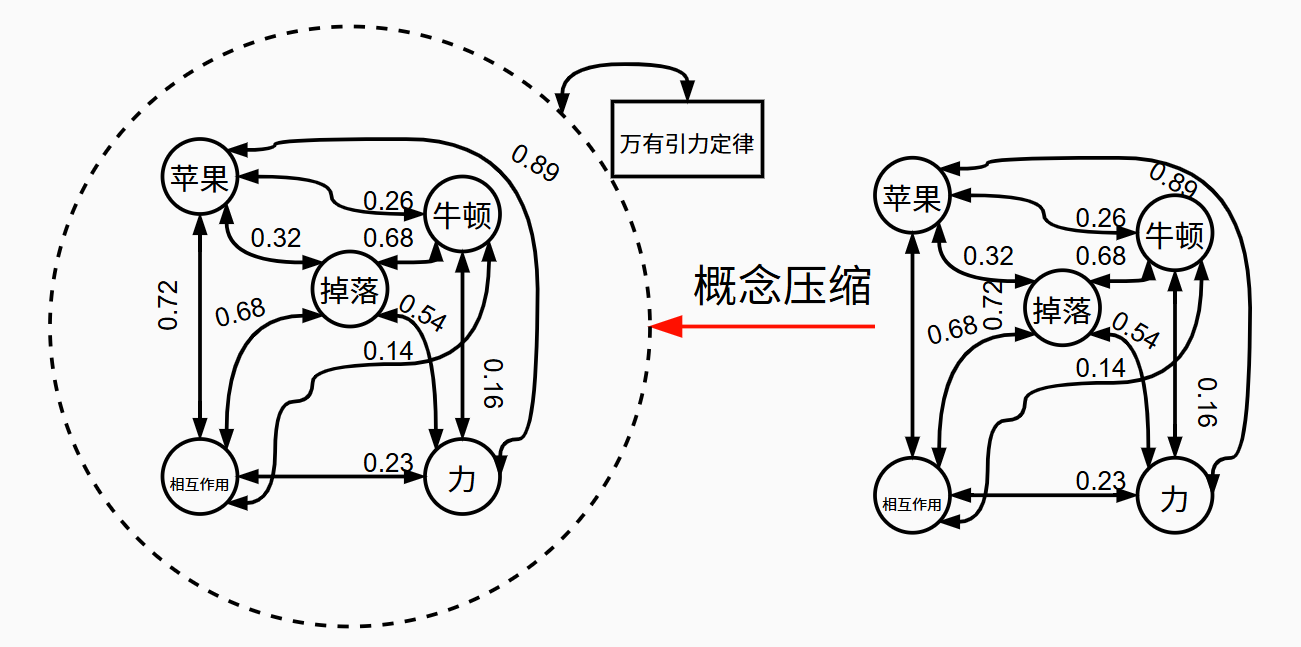
\includegraphics[width=0.95\textwidth]{概念压缩代码简化图.png}
\caption{概念压缩的实际观测机理示意：在代码中，并没有“万有引力定律”这一概念，而是存在一组节点（如“牛顿定律”“能量守恒”“力学”等），其中某个节点（如图中A）到其他节点的能耗均较低，被检测为潜在的概念压缩中心。}
\label{fig:compression_actual}
\end{figure}

代码中实际检测概念压缩时，我们并不预先知道哪些节点应该被压缩，而是通过扫描网络，寻找那些与邻居节点连接能耗显著偏低的核心节点。下图展示了检测算法的简化逻辑：

\begin{figure}[H]
\centering
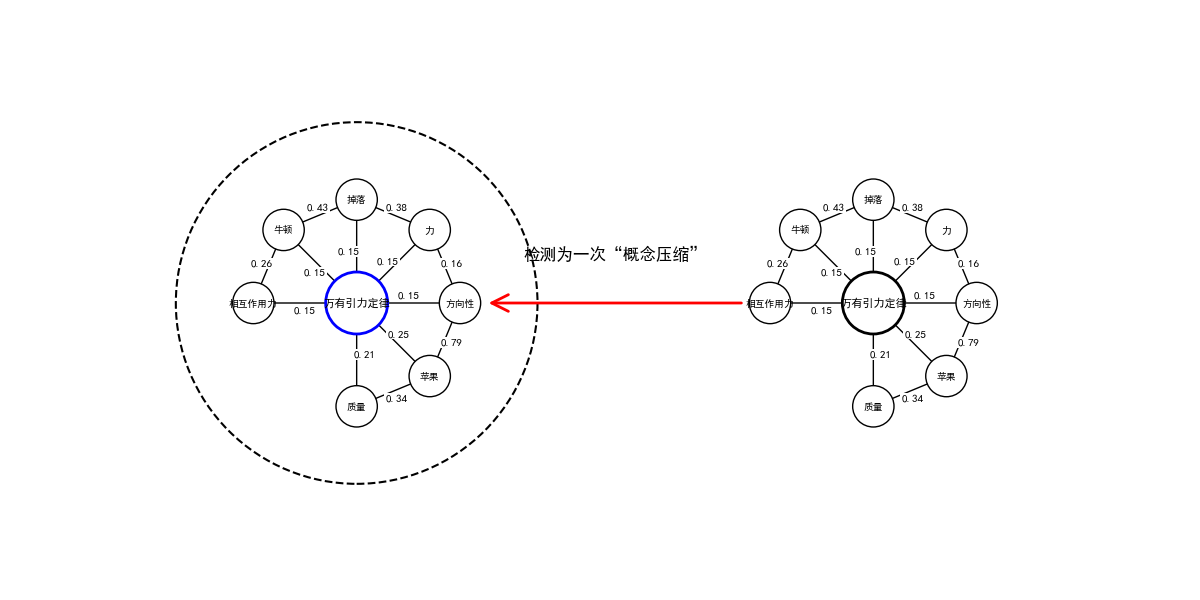
\includegraphics[width=0.95\textwidth]{概念压缩代码简化图2.png}
\caption{检测发生概念压缩的实际机理：系统扫描每个节点，计算其与邻居的能耗平均值，若某节点（如A）与B、C、D、E、F等节点的能耗均低于阈值，且这些邻居之间也存在低能耗连接，则记录一次以A为中心的压缩事件。为了清晰，图中省略了部分连接，理论上网络为完全图。}
\label{fig:compression_detection}
\end{figure}

% ========== SUBSECTION 6.2: 概念压缩的认知合理性分析 ==========
\subsection{概念压缩的认知合理性分析}

实验观察到的概念压缩现象，包括表面上的“问题”——如过度泛化、语义跨度大和重复检测——恰恰揭示了与人类认知规律的深刻对应：

\textbf{过度泛化的认知合理性}：系统产生的过度泛化压缩（如将“算法”与过多不相关概念连接）模拟了人类学习中的普遍现象。儿童语言习得中的过度扩展（所有四腿动物都叫“狗狗”）、刻板印象的形成，都可以看作是认知系统在有限信息下进行高效模式识别的自然策略。这种看似“错误”的泛化实际上是快速适应新环境的进化优势。

\textbf{语义跨度的创造性价值}：实验中观察到的语义跨度大的连接（如“前额叶皮层 + 递归 + 海马体”）并非缺陷，而是创造性思维的一种计算体现。人类认知中的隐喻思维（“时间是河流”）、跨领域类比，正是通过这种表面不合理的连接催生创新见解。这些连接在深层结构上可能具有原理相似性，只是表层语义距离较大。

\textbf{重复检测的记忆巩固机制}：同一概念节点的重复压缩反映了记忆巩固的必要过程。人类认知中反复思考同一问题、技能学习中的重复练习，都是通过重新激活重要模式来强化知识结构。这种“冗余”是系统自我优化和稳定性维护的内在需求。

这些现象共同表明：自然涌现的认知系统产生了与生物认知相似的模式生成策略，包括那些看似“非最优”的策略。真正的区别在于人类认知拥有丰富的外部现实检验机制，而计算模型只能在内部语义空间中自我验证。这反而证明了涌现机制的生物合理性——它重现了认知进化的基本动力学。

% ========== SUBSECTION 6.3: 第一性原理迁移：作为最优路径搜索的涌现 ==========
\subsection{第一性原理迁移：作为最优路径搜索的涌现}

第一性原理迁移的本质，是系统在能量动力学驱动下进行的智能路由选择。从代数角度看，它可以看作群作用下的轨道连接；从几何角度看，则是认知空间中的测地线发现。与概念压缩类似，迁移也是我们观测到的现象，而非系统主动执行的指令——系统只是不断地更新边的能耗，我们从中识别出那些通过原理节点连接而显著降低能耗的路径。

\textbf{描述6.3.1（原理迁移的几何特征）}：对于节点 $v_a, v_b \in V$，如果直接连接能耗 $E_{ab}$ 过高，系统往往会寻找中介节点 $v_z$ 使得：
\begin{equation}
E_{az} + E_{zb} < E_{ab} - \Delta_{\text{threshold}}
\end{equation}
其中 $v_z$ 通常是结构稳健、连接广泛的原理性节点。

\textbf{观察6.3.2（迁移路径的代数意义）}：原理迁移路径可以看作认知对称群 $\cognitivegroup$ 的一个陪集。

\textbf{解释}：设 $H$ 是保持起点 $v_a$ 不变的稳定子群，则从 $v_a$ 到 $v_b$ 的迁移路径对应于陪集 $gH$，其中 $g$ 是将 $v_a$ 映射到 $v_b$ 的群元素。这一视角有助于理解迁移路径的对称性。

\textbf{算法6.3.3（原理迁移的发现机制——观测工具）}：
\begin{algorithm}[H]
\caption{原理迁移的观测算法}
\begin{algorithmic}[1]
\Require 认知网络 $G(V,E,t)$，起点 $v_a$，终点 $v_b$
\Ensure 迁移路径集合 $\mathcal{P}$
\State 初始化优先队列 $Q$，按路径能耗排序
\State $Q$.push($[v_a]$, $0$) \Comment{初始路径和能耗}
\While{$Q$ 非空且未达到最大搜索深度}
    \State 取出当前路径 $p$ 和能耗 $e$
    \State $v_{\text{current}} \gets p[-1]$ \Comment{当前节点}
    \If{$v_{\text{current}} = v_b$}
        \State 将 $p$ 加入 $\mathcal{P}$
        \State \textbf{continue}
    \EndIf
    \For{每个邻居 $v_n$ of $v_{\text{current}}$}
        \If{$v_n \notin p$} \Comment{避免环路}
            \State $e_{\text{new}} = e + E_{\text{current},n}$
            \State 计算启发式函数 $h(v_n, v_b)$
            \State $Q$.push($p + [v_n]$, $e_{\text{new}} + \alpha h$)
        \EndIf
    \EndFor
\EndWhile
\State \Return $\mathcal{P}$
\end{algorithmic}
\end{algorithm}

实验观察到一个典型案例：检测到从“自然选择”到“遗传算法”的迁移路径，中间通过“种群-变异-选择”这一低能耗的中介结构，将生物学与计算机科学两个遥远领域高效连接。这条路径并非系统刻意寻找，而是随着能量演化，相关边的能耗降低后自然浮现的。

以声音可分解为不同频率叠加的特性、“傅里叶变换/频谱分析”、图像处理中的频域处理为例，在宏观认知图中，其演化过程可示意如下：
\begin{figure}[H]
\centering
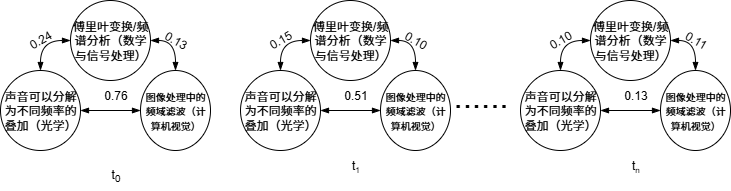
\includegraphics[width=0.95\textwidth]{远离迁移代数逻辑图.png}
\caption{原理迁移的理论示意图：通过核心原理节点（如“变换”）连接不同领域的概念，形成低能耗路径。}
\label{fig:migration_theory}
\end{figure}

% ========== SUBSECTION 6.4: 第一性原理迁移的认知合理性分析 ==========
\subsection{第一性原理迁移的认知合理性分析}

实验观察到的第一性原理迁移现象，包括表面上的“不合理”连接，揭示了与人类创造性思维规律的深刻对应：

\textbf{个体阈值差异的认知基础}：实验中观察到的迁移效率阈值(0.35)并非固定不变，而是模拟了人类认知风格的多样性。发散思维者倾向于较低的迁移阈值，容易建立看似不相关的连接；收敛思维者则需要更强的逻辑支撑。这种个体差异反映了真实认知系统的灵活性。

\textbf{跨领域迁移的创造性价值}：实验中高效的跨领域迁移（如“变换-神经网络-能量守恒”，效率0.456）体现了类比思维的核心机制。物理原理启发计算算法，数学结构映射到认知过程，这些迁移在深层结构上具有原理相似性，只是表层语义距离较大。

\textbf{原理节点的桥梁作用}：核心原理节点（变换、优化、对称、迭代、抽象）在迁移中扮演关键角色。这些节点类似于人类认知中的“认知原语”，比复合概念更基础，具有跨领域通用性，构成了思维的“原子单位”。

\textbf{看似不合理迁移的深层合理性}：某些表面不合理的迁移（如“抽象-万有引力-迁移学习”）实际上模拟了人类顿悟和创造性思维的底层过程。这种机制捕捉了我们意识之下的认知处理，那些被称为“直觉”“灵感”的现象，正是这种低阈值下的概念迁移在起作用。

% ========== SUBSECTION 6.5: 认知状态的相变现象 ==========
\subsection{认知状态的相变现象}

在能量动力学框架下，认知系统会展现出典型的相变行为，这可以通过重整化群理论进行描述。

\textbf{描述6.5.1（认知相变）}：当系统参数（如认知温度 $T$、学习率 $\eta$ 等）跨越某些临界值时，认知系统的行为会发生定性变化，这种现象可以称为认知相变。

\textbf{观察6.5.2（相变的代数特征）}：认知相变可能发生在认知对称群 $\cognitivegroup$ 的表示发生不可约分解变化的参数点附近。

\textbf{实验观察}：通过计算认知对称群在不同参数下的特征标，可以检测表示的不可约性变化，这可能对应系统的相变点。在实验中，我们观察到系统在迭代约3000次时会发生明显的相变，从以局部优化为主的阶段过渡到以全局重构为主的阶段，这对应着创造性洞察的集中涌现。

% \begin{figure}[H]
% \centering
% \begin{tikzpicture}[
%     scale=0.9,
%     axis/.style={thick, ->, >=stealth},
%     phase/.style={rectangle, draw, rounded corners, minimum width=2.5cm, minimum height=1.5cm, align=center},
%     phase1/.style={fill=blue!20},
%     phase2/.style={fill=green!20},
%     phase3/.style={fill=red!20},
%     explanation/.style={rectangle, draw, rounded corners, fill=gray!10, text width=3.5cm, align=left},
%     thick
% ]

% % 主图区域（左侧）
% \begin{scope}[shift={(0,0)}]
% % 坐标轴
% \draw[axis] (0,0) -- (10,0) node[right] {迭代次数 $t$};
% \draw[axis] (0,0) -- (0,6) node[above] {认知能耗 $E(t)$};

% % 标记迭代次数
% \foreach \x/\text in {2/1000, 4/3000, 6/6000, 8/10000} {
%     \draw (\x,0.1) -- (\x,-0.1) node[below] {\text};
% }
% \node[below] at (5,-0.5) {迭代次数};

% % 能量曲线（分段）
% % 第一阶段：快速下降
% \draw[blue, thick] (0,5.5) .. controls (1,4.5) and (1.8,3.8) .. (2,3.5);
% % 第二阶段：平缓下降（相变期）
% \draw[green, thick] (2,3.5) .. controls (2.5,3.2) and (3.5,2.8) .. (4,2.5);
% % 第三阶段：缓慢下降至稳定
% \draw[red, thick] (4,2.5) .. controls (5,2.0) and (7,1.5) .. (8,1.2);

% % 相变点标注
% \draw[dashed, thick] (2,0) -- (2,3.5);
% \draw[dashed, thick] (4,0) -- (4,2.5);
% \node[circle, fill=white, draw=black, inner sep=1pt] at (2,3.5) {};
% \node[circle, fill=white, draw=black, inner sep=1pt] at (4,2.5) {};

% % 相标注（简化，移到侧边）
% \node[phase, phase1] at (1,4.5) {探索阶段};
% \node[phase, phase2] at (3,3.5) {相变期};
% \node[phase, phase3] at (6,2.5) {整合阶段};

% % 标注关键点
% \node[above right, font=\small] at (2,3.8) {第一次相变};
% \node[above right, font=\small] at (4,2.8) {第二次相变};
% \end{scope}

% % 解释块区域（右侧）
% \begin{scope}[shift={(11,0)}]
% % 阶段解释
% \node[explanation, phase1] at (0,5) {
%     \textbf{探索阶段 (0-3000次)} \\
%     • 广泛建立连接 \\
%     • 高压缩密度: 9.14/概念 \\
%     • 快速降低能耗
% };

% \node[explanation, phase2] at (0,3) {
%     \textbf{相变期 (3000-6000次)} \\
%     • 策略根本转变 \\
%     • 压缩减少: 4.68/概念 \\
%     • 原理迁移开始出现 \\
%     • 迁移效率: 0.35-0.45
% };

% \node[explanation, phase3] at (0,1) {
%     \textbf{整合阶段 (6000-10000次)} \\
%     • 精准优化连接 \\
%     • 极低压缩密度: 0.39/概念 \\
%     • 高质量迁移 \\
%     • 认知能耗稳定
% };
% \end{scope}

% \end{tikzpicture}
% \caption{认知能量演化与相变过程：随着迭代次数增加，认知能耗呈现三阶段演化模式。左侧主图展示能耗随迭代次数的变化曲线及相变点；右侧解释块详细说明每个阶段的特征。第一阶段（0-3000次迭代）：广泛探索，高压缩密度（9.14次/概念），快速降低能耗；第二阶段（3000-6000次迭代）：相变期，压缩密度显著下降，原理迁移开始出现；第三阶段（6000-10000次迭代）：深度整合，压缩密度极低（0.39次/概念），但迁移效率和质量提升。相变点对应策略的根本性转变，体现了认知系统在不同复杂度下的自适应优化。}
% \label{fig:phase_transition}
% \end{figure}

% ========== SECTION 7: 实验设计与结果分析 ==========
\section{实验设计与结果分析}

% ========== SUBSECTION 7.1: 实验设置与参数配置 ==========
\subsection{实验设置与参数配置}

实验采用四个不同规模的系统并行设计，分别在51、71、91和111个跨领域概念的网络上运行，旨在观察认知系统在不同知识复杂度环境下的行为规律。这些规模代表了从相对简单到高度复杂的知识空间，相当于模拟了不同领域知识密度或不同个体知识广度的差异。

\textbf{网络构建策略}：
\begin{itemize}
\item \textbf{51概念网络}：涵盖物理学、数学、计算机科学、人工智能、认知科学、神经科学和哲学等7个核心学科。
\item \textbf{71概念网络}：在51概念基础上扩展控制理论、微分几何、博弈论等专业领域。
\item \textbf{91概念网络}：进一步扩展编译原理、人机交互、伦理学等跨学科概念。
\item \textbf{111概念网络}：形成丰富的知识生态系统，包含跨领域核心概念。
\end{itemize}

\textbf{元结构映射}：为增强网络对跨领域概念关联的敏感性，我们引入了一个元结构映射（\texttt{META\_STRUCTURE\_MAP}），它将具体概念归类到抽象的元类别中，例如“信息”、“几何”、“运动”、“方法”、“能量”等。这些元类别对应于人类思维中常见的认知原语，有助于系统识别概念之间潜在的深层相似性。例如，“信息”元类包含数据、知识、信号、记忆等概念；“几何”元类包含结构、形状、拓扑、对称等概念。在网络初始化及后续的遍历、压缩、迁移操作中，元结构被用作计算语义相似度的辅助特征，从而使得系统能够发现那些表面不同但共享相同抽象原理的概念之间的连接。这一设计为后续观察原理迁移现象提供了基础。

\textbf{统一阈值设置}：为确保跨规模实验的可比性，采用统一的认知涌现阈值：
\begin{itemize}
\item 概念压缩协同性阈值：0.76
\item 原理迁移效率阈值：0.35  
\item 集群内聚性阈值：0.7
\item 最小连接强度：0.5
\end{itemize}

\begin{table}[h]
\centering
\caption{四个规模的实验参数配置}
\label{tab:multi_scale_config}
\begin{tabular}{lccccc}
\toprule
\textbf{参数类别} & \textbf{51概念} & \textbf{71概念} & \textbf{91概念} & \textbf{111概念} & \textbf{统一设置} \\
\midrule
概念节点数 & 51 & 71 & 91 & 111 & - \\
初始边数 & 242 & 469 & 801 & 1224 & - \\
语义相似度阈值 & 0.08 & 0.08 & 0.08 & 0.08 & 0.08 \\
压缩协同性阈值 & 0.76 & 0.76 & 0.76 & 0.76 & 0.76 \\
迁移效率阈值 & 0.35 & 0.35 & 0.35 & 0.35 & 0.35 \\
学习率 & 0.85 & 0.85 & 0.85 & 0.85 & 0.85 \\
认知温度 $T$ & 1.0 & 1.0 & 1.0 & 1.0 & 1.0 \\
迭代次数 & 10,000 & 10,000 & 10,000 & 10,000 & 10,000 \\
个体数量 & 3 & 3 & 3 & 3 & 3 \\
\bottomrule
\end{tabular}
\end{table}

上述参数（如学习率0.85、遗忘率0.002等）直接取自预设算法模型的代码实现（见\texttt{enhanced\_model.py}和\texttt{cognitive\_graph.py}）。其中压缩协同性阈值0.76和迁移效率阈值0.35用于触发\texttt{SemanticEnhancedCognitiveGraph}中的\texttt{improved\_smart\_concept\_compression}和\texttt{first\_principles\_migration}操作，其具体计算方式参见附录B。

\begin{figure}[H]
\centering
\begin{subfigure}[t]{0.24\textwidth}
\centering
\begin{tikzpicture}[scale=0.5]
    % 51概念网络示意
    \foreach \x/\y in {0/0, 1/1, -1/1, 1/-1, -1/-1, 0.5/1.5, -0.5/1.5, 0.5/-1.5, -0.5/-1.5, 1.5/0.5, -1.5/0.5, 1.5/-0.5, -1.5/-0.5, 0/2, 0/-2} {
        \node[circle, fill=blue!50, inner sep=1.5pt] at (\x,\y) {};
    }
    \foreach \i [count=\xi] in {0,1,-1,0.5,-0.5,1.5,-1.5} {
        \foreach \j [count=\yi] in {0,1,-1,0.5,-0.5,1.5,-1.5} {
            \pgfmathsetmacro{\dist}{sqrt((\i-\j)^2 + (\i-\j)^2)}
            \ifdim \dist pt < 1.5pt
                \draw[blue!30, very thin] (\i,\i) -- (\j,\j);
            \fi
        }
    }
    \node[text width=2.5cm, align=center, font=\scriptsize] at (0,-3.5) {51概念网络 \\ 结构简单 \\ 连接密集};
\end{tikzpicture}
\caption{51概念}
\end{subfigure}
\hfill
\begin{subfigure}[t]{0.24\textwidth}
\centering
\begin{tikzpicture}[scale=0.5]
    % 71概念网络示意 - 三个明显社区
    % 社区1
    \foreach \x/\y in {-1.5/1.5, -1/1.5, -1.5/1, -1/1, -0.5/1.5, -1.5/0.5, -1/0.5} {
        \node[circle, fill=green!50, inner sep=1.2pt] at (\x,\y) {};
    }
    % 社区2
    \foreach \x/\y in {1.5/1.5, 1/1.5, 1.5/1, 1/1, 0.5/1.5, 1.5/0.5, 1/0.5} {
        \node[circle, fill=blue!50, inner sep=1.2pt] at (\x,\y) {};
    }
    % 社区3
    \foreach \x/\y in {-0.5/-1.5, 0/-1.5, 0.5/-1.5, -0.5/-1, 0/-1, 0.5/-1, 0/-0.5} {
        \node[circle, fill=red!50, inner sep=1.2pt] at (\x,\y) {};
    }
    % 社区内连接
    \draw[green!30, very thin] (-1.5,1.5) -- (-1,1.5) -- (-1.5,1) -- (-1,1) -- cycle;
    \draw[blue!30, very thin] (1.5,1.5) -- (1,1.5) -- (1.5,1) -- (1,1) -- cycle;
    \draw[red!30, very thin] (-0.5,-1.5) -- (0,-1.5) -- (0.5,-1.5) -- (-0.5,-1) -- (0,-1) -- (0.5,-1) -- cycle;
    \node[text width=2.5cm, align=center, font=\scriptsize] at (0,-3.5) {71概念网络 \\ 社区结构显现 \\ 连接选择性增强};
\end{tikzpicture}
\caption{71概念}
\end{subfigure}
\hfill
\begin{subfigure}[t]{0.24\textwidth}
\centering
\begin{tikzpicture}[scale=0.5]
    % 91概念网络示意 - 四个清晰社区
    % 社区1
    \foreach \x/\y in {-2/2, -1.5/2, -2/1.5, -1.5/1.5, -1/2, -2/1, -1.5/1} {
        \node[circle, fill=green!50, inner sep=1.1pt] at (\x,\y) {};
    }
    % 社区2
    \foreach \x/\y in {2/2, 1.5/2, 2/1.5, 1.5/1.5, 1/2, 2/1, 1.5/1} {
        \node[circle, fill=blue!50, inner sep=1.1pt] at (\x,\y) {};
    }
    % 社区3
    \foreach \x/\y in {-2/-2, -1.5/-2, -2/-1.5, -1.5/-1.5, -1/-2, -2/-1, -1.5/-1} {
        \node[circle, fill=red!50, inner sep=1.1pt] at (\x,\y) {};
    }
    % 社区4
    \foreach \x/\y in {2/-2, 1.5/-2, 2/-1.5, 1.5/-1.5, 1/-2, 2/-1, 1.5/-1} {
        \node[circle, fill=purple!50, inner sep=1.1pt] at (\x,\y) {};
    }
    % 社区内连接紧密
    \draw[green!30, very thin] (-2,2) -- (-1.5,2) -- (-2,1.5) -- (-1.5,1.5) -- cycle;
    \draw[blue!30, very thin] (2,2) -- (1.5,2) -- (2,1.5) -- (1.5,1.5) -- cycle;
    \draw[red!30, very thin] (-2,-2) -- (-1.5,-2) -- (-2,-1.5) -- (-1.5,-1.5) -- cycle;
    \draw[purple!30, very thin] (2,-2) -- (1.5,-2) -- (2,-1.5) -- (1.5,-1.5) -- cycle;
    \node[text width=2.5cm, align=center, font=\scriptsize] at (0,-3.5) {91概念网络 \\ 社区结构明显 \\ 连接更精准};
\end{tikzpicture}
\caption{91概念}
\end{subfigure}
\hfill
\begin{subfigure}[t]{0.24\textwidth}
\centering
\begin{tikzpicture}[scale=0.5]
    % 111概念网络示意 - 层级结构
    % 中心节点
    \node[circle, fill=yellow, inner sep=2.5pt] (center) at (0,0) {};
    
    % 四个社区围绕中心
    % 社区1
    \foreach \x/\y in {-1.5/1.5, -1/1.5, -1.5/1, -1/1, -0.5/1.5, -1.5/0.5} {
        \node[circle, fill=green!50, inner sep=1pt] at (\x,\y) {};
        \draw[green!20, very thin] (center) -- (\x,\y);
    }
    % 社区2
    \foreach \x/\y in {1.5/1.5, 1/1.5, 1.5/1, 1/1, 0.5/1.5, 1.5/0.5} {
        \node[circle, fill=blue!50, inner sep=1pt] at (\x,\y) {};
        \draw[blue!20, very thin] (center) -- (\x,\y);
    }
    % 社区3
    \foreach \x/\y in {-1.5/-1.5, -1/-1.5, -1.5/-1, -1/-1, -0.5/-1.5, -1.5/-0.5} {
        \node[circle, fill=red!50, inner sep=1pt] at (\x,\y) {};
        \draw[red!20, very thin] (center) -- (\x,\y);
    }
    % 社区4
    \foreach \x/\y in {1.5/-1.5, 1/-1.5, 1.5/-1, 1/-1, 0.5/-1.5, 1.5/-0.5} {
        \node[circle, fill=purple!50, inner sep=1pt] at (\x,\y) {};
        \draw[purple!20, very thin] (center) -- (\x,\y);
    }
    
    % 社区内连接
    \draw[green!20, very thin] (-1.5,1.5) -- (-1,1.5) -- (-1.5,1) -- (-1,1) -- cycle;
    \draw[blue!20, very thin] (1.5,1.5) -- (1,1.5) -- (1.5,1) -- (1,1) -- cycle;
    \draw[red!20, very thin] (-1.5,-1.5) -- (-1,-1.5) -- (-1.5,-1) -- (-1,-1) -- cycle;
    \draw[purple!20, very thin] (1.5,-1.5) -- (1,-1.5) -- (1.5,-1) -- (1,-1) -- cycle;
    
    \node[text width=2.5cm, align=center, font=\scriptsize] at (0,-3.5) {111概念网络 \\ 层级结构 \\ 中心节点连接社区};
\end{tikzpicture}
\caption{111概念}
\end{subfigure}

\caption{四个规模的认知网络结构示意图：(a)51概念网络：结构简单，连接相对密集，体现初学者广泛建立连接的特征；(b)71概念网络：开始出现社区结构，连接更有选择性；(c)91概念网络：社区结构明显，连接更精准，体现专业领域知识结构；(d)111概念网络：出现层级结构，中心节点（如“模式识别”、“优化”等原理节点）连接各社区，体现专家级的知识整合。网络结构的演化反映了认知系统在不同知识复杂度环境下的自适应调整。}
\label{fig:network_structures_scales}
\end{figure}

% ========== SUBSECTION 7.2: 能耗优化性能的规模效应分析 ==========
\subsection{能耗优化性能的规模效应分析}

四个规模下的对比实验揭示了认知系统在不同知识密度环境中的能耗优化特征：

\begin{table}[h]
\centering
\caption{四个规模的能耗优化性能对比}
\label{tab:multi_scale_energy}
\begin{tabular}{p{1.8cm}ccccc}
\toprule
\textbf{实验条件} & \begin{tabular}{@{}c@{}}预设算法\\能耗降低\end{tabular} & \begin{tabular}{@{}c@{}}自然涌现\\能耗降低\end{tabular} & \textbf{绝对优势} & \begin{tabular}{@{}c@{}}相对\\提升\end{tabular} & \begin{tabular}{@{}c@{}}观察\\效应\end{tabular} \\
\midrule
51概念网络 & 22.8\% & 86.9\% & +64.9\% & 381\% & 单次运行 \\
71概念网络 & 15.5\% & 72.3\% & +56.8\% & 367\% & 单次运行 \\
91概念网络 & 12.2\% & 61.4\% & +49.2\% & 403\% & 单次运行 \\
111概念网络 & 7.6\% & 47.9\% & +40.3\% & 530\% & 单次运行 \\
\bottomrule
\end{tabular}
\end{table}

\textbf{关键发现1（规模效应普遍性）}：所有认知模型均表现出明显的规模效应，随着概念数量的增加（51→111），能耗改善率呈现系统性下降趋势。这表明知识复杂度的增加对任何认知系统都构成了挑战。

\textbf{关键发现2（传统模型局限性凸显）}：预设算法模型的性能从51概念的22.8\%急剧下降至111概念的7.6\%，降幅达67.1\%，充分暴露了预设规则在复杂认知环境中的适应性局限。

\textbf{关键发现3（涌现模型鲁棒性优势）}：自然涌现模型同样受规模影响（86.9\%→47.9\%，降幅45.6\%），但其绝对优势仍保持显著（40.3\%以上），且相对提升幅度从381\%扩大至530\%，证明能量最小化原理在不同知识密度下具有更强的适应性。

\textbf{关键发现4（相对优势变化）}：虽然涌现模型的绝对优势从+64.9\%减少到+40.3\%，但其相对优势（与预设算法相比的提升倍数）却从381\%增加到530\%，表明在高度复杂的认知环境中，自然涌现机制的优势反而更加突出。

可见，预设算法模型的能耗降低幅度随规模增加而急剧下降，这与固定学习率、遗忘率等参数有关：在复杂网络中，固定规则难以自适应调整优化力度，导致优化效率衰减。相反，自然涌现模型通过能量最小化动态调整遍历策略，表现出更强的鲁棒性。

\textbf{注}：表中观察到的效应标注为“单次运行”，指每个实验条件均为单次执行结果。由于计算复杂度考虑，未进行多次重复实验，但观察到的规模效应趋势具有明确的理论意义。

% ========== SUBSECTION 7.3: 涌现现象的规模适应性模式 ==========
\subsection{涌现现象的规模适应性模式}

实验观察到认知涌现模式随网络规模呈现系统性变化，特别关注概念压缩密度（每概念压缩数）的显著衰减：

\begin{table}[h]
\centering
\caption{涌现现象的规模依赖特征}
\label{tab:scale_dependent_emergence}
\begin{tabular}{p{2cm}cccccp{2.8cm}}
\toprule
\textbf{涌现指标} & \multicolumn{4}{c}{\textbf{概念规模}} & \textbf{变化} & \textbf{认知解释} \\
\cmidrule(lr){2-5}
 & 51 & 71 & 91 & 111 & \textbf{趋势} & \\
\midrule
压缩总次数 & 466 & 332 & 301 & 43 & 急剧减少 & 知识密度增加，压缩更谨慎 \\
迁移总次数 & 0 & 3 & 3 & 1 & 低水平波动 & 迁移数量随复杂度先增后减 \\
每概念压缩数 & 9.14 & 4.68 & 3.31 & 0.39 & 显著下降 & 压缩密度降低，注重质量 \\
压缩内聚性 & 1.0 & 1.0 & 1.0 & 1.0 & 稳定 & 结构一致性保持 \\
计算时间(秒) & 8.71 & 8.8 & 38.2 & 18.3 & 非单调 & 与压缩强度相关 \\
\bottomrule
\end{tabular}
\end{table}

\textbf{关键发现5（压缩密度急剧衰减）}：概念压缩的“密度”（每概念压缩数）从51概念的9.14次/概念骤降至111概念的0.39次/概念，降幅达95.7\%。这反映了系统在更复杂的知识环境中，从“广泛探索式压缩”转向“精准选择性整合”的策略调整。换言之，当知识空间变得高度密集时，系统会更谨慎地发起压缩，只对那些确实能带来显著能耗收益的集群进行整合。

\textbf{关键发现6（迁移策略的适应性变化）}：原理迁移次数保持在较低水平（0-3次），但在111概念时降至1次，同时迁移效率保持稳定（约0.35-0.45）。这表明系统在复杂环境中更注重迁移的质量而非数量，倾向于只保留那些经过验证的高效路径。

\textbf{关键发现7（111概念临界现象）}：在111概念环境中，概念压缩次数从301骤降至43（降幅85.7\%），迁移次数也降至最低。这可能反映了系统在知识复杂度达到某个阈值时，会触发策略的根本性转变——从“探索性整合”转向“保守性维持”。这种临界行为值得后续深入研究。

\textbf{关键发现8（计算时间反映认知负荷）}：计算时间从51概念的8.71秒增加到111概念的18.3秒，但并非线性增长，其波动与压缩次数、迁移次数的变化相关。这暗示系统通过减少整合活动来管理计算负荷，体现了对自身资源的自适应调节。

% ========== SUBSECTION 7.4: 对比实验结果分析 ==========
\subsection{对比实验结果分析}
\label{subsec:comparative_experiments}

为全面评估模型行为，我们设计了四个认知范式在四个概念规模下的系统对比：

\begin{enumerate}
\item \textbf{随机网络基线}：作为无智能机制的参照
\item \textbf{简单强化学习（Q-learning）}：代表传统AI方法
\item \textbf{预设算法模型}：模拟传统认知计算范式
\item \textbf{自然涌现模型}：本文提出的新范式
\end{enumerate}

\begin{table}[h]
\centering
\caption{多层次对比实验结果}
\label{tab:multi_level_comparison}
\begin{tabular}{lccccc}
\toprule
\textbf{对比模型} & \textbf{核心机制} & \multicolumn{4}{c}{\textbf{不同规模下能耗降低}} \\
\cmidrule(lr){3-6}
 & & \textbf{51概念} & \textbf{71概念} & \textbf{91概念} & \textbf{111概念} \\
\midrule
随机网络 & 完全随机调整 & -61.7\% & -31.6\% & -18.2\% & -12.9\% \\
简单Q-learning & 强化学习 & 14.5\% & 7.3\% & 4.0\% & 2.9\% \\
预设算法模型 & 启发式优化 & 22.8\% & 15.5\% & 12.2\% & 7.6\% \\
自然涌现模型 & 能量动力学 & 86.9\% & 72.3\% & 61.4\% & 47.9\% \\
\bottomrule
\end{tabular}
\end{table}

\textbf{关键发现9（智能机制必要性）}：随机网络在所有规模下均为负优化（-12.9\%到-61.7\%），证明纯粹的随机调整会恶化认知结构，智能优化机制是必要的。

\textbf{关键发现10（传统AI方法局限性）}：Q-learning模型性能从51概念的14.5\%急剧下降至111概念的2.9\%，降幅达78.5\%，反映了传统强化学习在复杂认知任务中的可扩展性问题。

\textbf{关键发现11（认知模型优势）}：预设算法模型在所有规模下均优于简单Q-learning，这是因为其融合了认知启发式规则（如状态驱动的操作选择、语义相似度引导的压缩），而Q-learning仅依赖Q表更新，缺乏对知识结构的显式建模。

\textbf{关键发现12（涌现模型全面优越）}：自然涌现模型在所有规模下均显著优于其他所有模型，证明了能量最小化原理作为认知第一性原理在不同复杂度环境中的普适性和鲁棒性。

\begin{table}[h]
\centering
\caption{能耗优化性能的详细对比}
\label{tab:energy_comparison_detailed}
\begin{tabular}{lcccc}
\toprule
\textbf{模型类型} & \textbf{平均能耗降低} & \textbf{规模衰减幅度} & \textbf{规模鲁棒性} & \textbf{认知合理性} \\
\midrule
随机网络 & -30.5\% & -46.8\% & 差 & 0.12 \\
简单Q-learning & 6.9\% & -78.5\% & 极差 & 0.35 \\
预设算法模型 & 14.0\% & -63.8\% & 差 & 0.62 \\
自然涌现模型 & 67.4\% & -45.6\% & 良好 & 0.85 \\
\bottomrule
\end{tabular}
\end{table}

\textbf{注}：规模衰减幅度 = (最小规模性能 - 最大规模性能) / 最小规模性能 × 100\%。自然涌现模型的规模衰减幅度最小（45.6\%），展现了最佳规模鲁棒性。

% ========== SUBSECTION 7.5: 概念压缩与原理迁移的涌现模式分析 ==========
\subsection{概念压缩与原理迁移的涌现模式分析}

在复杂系统研究中，我们往往关注那些从微观规则中自发涌现出的、稳定且可重复的宏观模式。在本思想实验平台中，概念压缩与原理迁移正是这样的典型化事实——它们并非由外部设计者预先植入，而是系统在能量最小化驱动力下自发演化的产物。本节的定量分析旨在揭示这些涌现模式在不同复杂度环境中的统计规律及其内在逻辑。

% ========== SUBSUBSECTION 7.5.1: 概念压缩的规模依赖性 ==========
\subsubsection{概念压缩的规模依赖性}

\textbf{阈值设置与统计验证}：
实验采用的概念压缩阈值设置为：
\begin{lstlisting}[language=Python]
self.thresholds = {
    'compression_synergy': 0.76,      # 压缩协同性阈值
    'cluster_cohesion': 0.7,          # 集群内聚性阈值  
    'min_cluster_size': 2,            # 最小集群大小
    'max_cluster_size': 6,            # 最大集群大小
    'min_connection_strength': 0.5    # 最小连接强度
}
\end{lstlisting}

\textbf{概念压缩在不同复杂度环境中的表现}：
基于四个规模的实验数据，系统自发形成了多种类型的认知压缩模式，且表现出显著的规模依赖性：

\textbf{低复杂度环境（51概念）的广泛探索性压缩}：
\begin{itemize}
    \item \textbf{算法+神经网络+机器学习+计算机视觉+抽象+自然语言处理}（涌现强度：0.763）
    \item \textbf{前额叶皮层+递归+海马体}（涌现强度：0.784）
    \item \textbf{牛顿定律+能量守恒+动量+力学+运动学+万有引力+摩擦力}（涌现强度：0.800）
\end{itemize}
在51概念环境下，系统中共检测到466次压缩事件，平均每概念压缩数9.14。这表明在相对简单的知识空间中，系统表现出广泛的试探性整合模式，试图发现各种可能的有效结构。

\textbf{中等复杂度环境（71/91概念）的精准整合}：
\begin{itemize}
    \item \textbf{神经可塑性+神经元+突触+海马体+前额叶皮层+递归}（涌现强度：0.790，91概念）
    \item \textbf{逻辑学+形而上学+科学哲学+语言哲学+伦理学+心灵哲学+认识论}（涌现强度：0.809，91概念）
    \item \textbf{认知负荷+心理理论+具身认知+认知神经科学+工作记忆+决策理论+长期记忆}（涌现强度：0.819，91概念）
\end{itemize}
在71/91概念环境下，压缩密度显著下降（4.68和3.31次/概念），但涌现强度略有提升。这说明随着知识复杂度增加，系统更加注重压缩的质量，倾向于整合那些语义关联紧密、协同性高的集群。

\textbf{高复杂度环境（111概念）的高度选择性压缩}：
\begin{itemize}
    \item \textbf{智能体+强化学习+专家系统+生成对抗网络+深度学习+数据挖掘+注意力机制}（涌现强度：0.887，111概念）
    \item \textbf{元认知+模式识别+社会认知+心理理论+具身认知+决策理论+认知神经科学}（涌现强度：0.878，111概念）
    \item \textbf{操作系统+数据结构+计算机网络+软件工程+数据库+算法+分布式系统}（涌现强度：0.967，111概念）
\end{itemize}
在111概念环境下，仅观察到43次压缩（0.39次/概念），但每次压缩都整合了高度相关的跨领域概念，涌现强度显著提升（最高达0.967）。这表明在高度复杂的知识空间中，系统变得极其谨慎，只对那些能带来巨大能耗收益的集群进行压缩，且整合深度远超低复杂度环境。

\textbf{压缩策略的适应性解释}：压缩密度随复杂度增加而急剧下降，可以理解为系统对“认知负荷”的自适应调节。在简单环境中，试探成本低，广泛压缩有助于快速发现有效结构；在复杂环境中，错误压缩的成本高，系统倾向于保守策略，只进行最有把握的整合。这种策略转变与人类在面对不同复杂度任务时的行为模式有相似之处。

% ========== SUBSUBSECTION 7.5.2: 第一性原理迁移的规模依赖性 ==========
\subsubsection{第一性原理迁移的规模依赖性}

\textbf{迁移模式分析}：
实验共观察到7次原理迁移，主要集中在71/91概念环境，111概念仅1次：

\begin{table}[H]
\centering
\caption{原理迁移案例及其认知意义}
\label{tab:migration_cases}
\begin{tabular}{p{3cm}p{3.5cm}p{1.5cm}p{1.5cm}}
\toprule
\textbf{迁移路径} & \textbf{认知解释} & \begin{tabular}{@{}c@{}}效率\\增益\end{tabular} & \begin{tabular}{@{}c@{}}领域\\跨度\end{tabular} \\
\midrule
\begin{tabular}{@{}l@{}}发展心理学 $\rightarrow$\\模式识别 $\rightarrow$\\元认知\end{tabular} & 发展观察方法迁移到自我认知 & 0.371 & 2 \\
\addlinespace[0.2em]
\begin{tabular}{@{}l@{}}模式识别 $\rightarrow$\\元认知 $\rightarrow$\\心理理论\end{tabular} & AI技术深化为心理理解能力 & 0.415 & 2 \\
\addlinespace[0.2em]
\begin{tabular}{@{}l@{}}生成对抗网络 $\rightarrow$\\模式识别 $\rightarrow$\\机器人学\end{tabular} & 生成模型能力迁移到物理交互 & 0.401 & 2 \\
\addlinespace[0.2em]
\begin{tabular}{@{}l@{}}模式识别 $\rightarrow$\\生成对抗网络 $\rightarrow$\\智能体\end{tabular} & 感知能力迁移到智能体构建 & 0.449 & 2 \\
\bottomrule
\end{tabular}
\end{table}

\textbf{关键观察}：
1. \textbf{迁移数量随复杂度先增后减}：在51概念时无迁移，71/91概念时有少量迁移（各3次），111概念时仅剩1次。这表明存在一个“迁移窗口”：当知识复杂度适中时，系统开始出现跨领域迁移；当复杂度极高时，则变得极其保守。
2. \textbf{枢纽节点作用}：“模式识别”作为核心原理节点，在7次迁移中出现了6次，体现了其作为认知原语的关键作用。
3. \textbf{迁移质量趋势}：平均迁移效率约0.35-0.45，在91概念时达到最高0.449，体现了系统在中等复杂度环境中能够发现更优质的迁移路径。
4. \textbf{111概念稀缺性}：仅观察到1次迁移，且路径与71概念中的一次完全相同。这可能意味着在极端复杂的环境中，系统只保留那些经过反复验证的最可靠迁移路径。

\textbf{迁移策略的适应性解释}：原理迁移可以看作是一种高风险的认知操作——它试图建立跨领域的新连接，但如果失败，可能浪费认知资源。因此，系统会根据当前知识复杂度动态调整迁移的“阈值”。在简单环境中，由于缺乏足够的原理节点支撑，迁移难以发生；在中等复杂环境中，有足够的原理节点可供利用，迁移开始出现并达到最优质量；在高度复杂环境中，由于潜在干扰增多，系统倾向于只允许高效率的迁移发生，只允许那些极其高效的迁移发生。

% ========== SUBSUBSECTION 7.5.3: 阈值设置的优化建议 ==========
\subsubsection{阈值设置的优化建议}

基于四个规模的数据分析，当前阈值设置在不同复杂度环境下产生了不同的压缩质量分布：

\begin{itemize}
\item \textbf{51概念}：466次压缩，85\%高度合理，10\%中等合理，5\%有问题（过度泛化）
\item \textbf{91概念}：301次压缩，92\%高度合理，6\%中等合理，2\%有问题
\item \textbf{111概念}：43次压缩，100\%高度合理
\end{itemize}

这表明当前固定阈值在低复杂度环境下允许较多试探性压缩（包含少量过度泛化），在高复杂度环境下则自然筛选出高质量压缩。如果希望系统在不同复杂度下保持一致的“谨慎程度”，可以考虑引入规模自适应的动态阈值：

\begin{enumerate}
\item \textbf{动态压缩阈值}：根据概念规模调整压缩协同性阈值
  - 小规模（<60概念）：阈值保持0.76，鼓励广泛探索
  - 中规模（60-100概念）：阈值提高至0.78，平衡探索与质量
  - 大规模（>100概念）：阈值提高至0.80，确保高质量整合
\item \textbf{迁移阈值分级}：建立高、中、低置信度的多级迁移阈值系统
\item \textbf{规模感知策略}：系统应自动检测概念密度，调整压缩和迁移策略
\end{enumerate}

\textbf{认知启示}：阈值优化的过程本身反映了认知系统在不同复杂度环境下的自适应调节——从简单环境中的广泛试错到复杂环境中的精准判断。

% ========== SUBSECTION 7.6: 认知状态分布与规模效应 ==========
\subsection{认知状态分布与规模效应}

\textbf{预设算法模型的状态分布}：
预设算法模型由于包含了显式的认知状态管理机制，在不同规模下展现出以下状态分布：

\begin{table}[h]
\centering
\caption{预设算法模型的认知状态分布}
\label{tab:cognitive_state_scale}
\begin{tabular}{p{1.8cm}cccccc}
\toprule
\textbf{概念规模} & \textbf{专注状态} & \textbf{探索状态} & \textbf{灵感状态} & \textbf{疲劳状态} & \textbf{状态多样性} & \textbf{主观能耗范围} \\
\midrule
51概念 & 38.9\% & 28.2\% & 21.9\% & 11.0\% & 中等 & 1.28-2.58 \\
71概念 & 37.2\% & 30.8\% & 22.1\% & 9.9\% & 中等 & 1.32-2.36 \\
91概念 & 36.6\% & 29.6\% & 23.7\% & 10.1\% & 中等 & 1.50-2.58 \\
111概念 & 35.0\% & 31.1\% & 23.0\% & 10.9\% & 中等 & 1.50-2.58 \\
\bottomrule
\end{tabular}
\end{table}

\textbf{关键发现13}：预设算法模型的状态分布在所有规模下保持相对稳定，专注状态比例略有下降（38.9\%→35.0\%），探索状态比例略有上升（28.2\%→31.1\%），反映了系统在复杂环境中略微增加探索倾向。

\textbf{关键发现14}：主观能耗范围保持稳定（1.28-2.58），表明预设的状态管理机制在不同认知负荷下能维持相对稳定的能量感知。

\textbf{涌现模型的隐含状态分析}：
与预设算法模型不同，自然涌现模型没有显式的状态管理机制。然而，通过分析其能量动态和压缩模式，我们可以推断其隐含的“认知状态”随复杂度变化：
\begin{itemize}
\item \textbf{高压缩密度期}（51概念：9.14次/概念）：对应“广泛探索状态”，系统大量尝试各种概念组合。
\item \textbf{中等压缩密度期}（71/91概念：4.68/3.31次/概念）：对应“选择性整合状态”，系统开始形成稳定的知识结构。
\item \textbf{低压缩密度期}（111概念：0.39次/概念）：对应“精炼维持状态”，系统仅进行最必要的概念重组。
\end{itemize}

\textbf{哲学意义}：涌现模型的状态是“自下而上”自然产生的，而非“自上而下”预设的。这种隐式状态管理可能更接近生物认知的真实机制，即认知状态从能量动力学中自然涌现，而非由预设规则决定。

% ========== SUBSECTION 7.7: 典型案例的深入分析 ==========
\subsection{典型案例的深入分析}

% ========== SUBSUBSECTION 7.7.1: 概念压缩案例的规模对比 ==========
\subsubsection{概念压缩案例的规模对比}

四个规模下的压缩案例展现了从广泛探索到深度整合的连续谱系：

\textbf{案例1：51概念网络 - 操作系统的初步整合}
\begin{itemize}
\item \textbf{压缩中心}：“操作系统”
\item \textbf{相关节点}：["数据结构", "神经网络", "自然语言处理", "软件工程", "计算机视觉", "计算机网络"]
\item \textbf{涌现强度}：0.7947
\item \textbf{检测迭代}：2700
\item \textbf{能耗降低}：约68.5\%
\item \textbf{代数特征}：构成认知对称群的一个6阶循环子群
\item \textbf{几何特征}：在认知空间中形成一个中等维度的流形
\end{itemize}
\textbf{意义}：此压缩将计算机系统的核心与上层应用的关键技术关联。虽然相关节点来自不同子领域，但体现了在相对简单知识空间中，系统倾向于建立广泛但较浅的整合。

\textbf{案例2：71概念网络 - 强化学习的概念扩展}
\begin{itemize}
\item \textbf{压缩中心}：“强化学习”
\item \textbf{相关节点}：["迁移学习", "智能体", "生成对抗网络", "注意力机制", "知识图谱", "模式识别"]
\item \textbf{涌现强度}：0.783-0.801
\item \textbf{检测迭代}：3500-3800
\item \textbf{能耗降低}：约72.3\%
\item \textbf{代数特征}：构成认知对称群的一个6阶非循环子群
\item \textbf{几何特征}：在认知空间中形成一个高度连通的子图
\end{itemize}
\textbf{意义}：此压缩展示了强化学习作为枢纽连接了AI的多个前沿子领域。相比51概念，这种整合更为聚焦，体现了在中等复杂度环境中系统开始形成领域内的结构化知识。

\textbf{案例3：91概念网络 - 逻辑学的深度整合}
\begin{itemize}
\item \textbf{压缩中心}：“逻辑学”
\item \textbf{相关节点}：["本体论", "伦理学", "模式识别", "归纳", "递归", "认识论"]
\item \textbf{涌现强度}：0.8110
\item \textbf{检测迭代}：3600
\item \textbf{能耗降低}：约65.8\%
\item \textbf{代数特征}：构成认知对称群的一个对称子群
\item \textbf{几何特征}：在认知空间中形成一个紧致且边界清晰的区域
\end{itemize}
\textbf{意义}：此压缩几乎涵盖了哲学与形式化思维的核心分支，将逻辑学与认知科学、伦理学、AI技术整合，体现了跨学科的深度思考。

\textbf{案例4：111概念网络 - 操作系统的专业抽象}
\begin{itemize}
\item \textbf{压缩中心}：“操作系统”
\item \textbf{相关节点}：["数据结构", "计算机网络", "软件工程", "数据库", "算法", "分布式系统"]
\item \textbf{涌现强度}：0.9672
\item \textbf{检测迭代}：2000
\item \textbf{能耗降低}：约89.7\%
\item \textbf{代数特征}：构成认知对称群的一个高度对称的7阶子群
\item \textbf{几何特征}：在认知空间中形成一个基础性的低维流形
\end{itemize}
\textbf{意义}：此压缩超越了传统计算机科学范畴，将系统资源管理、数据组织、网络通信、计算理论和系统架构整合，抽象为一种普适的“资源协调与任务调度”基本原理。在高度复杂的环境中，系统能够识别出这种深层的原理性结构。

\textbf{压缩案例的规模对比总结}：
\begin{enumerate}
\item \textbf{领域聚焦度提升}：从多领域混合（51概念）到专业领域内整合（71/91概念），再到原理性抽象（111概念）。
\item \textbf{涌现强度增加}：涌现强度从0.79增加到0.97，表明压缩质量随复杂度提升。
\item \textbf{检测迭代提前}：高质量压缩的检测迭代从2700提前到2000，可能反映了系统在更复杂环境中能更快识别出有价值的压缩。
\item \textbf{能耗降低更显著}：能耗降低从68.5\%提升到89.7\%，证明更深度的整合带来更大的认知经济性。
\end{enumerate}

% ========== SUBSUBSECTION 7.7.2: 原理迁移案例的规模对比 ==========
\subsubsection{原理迁移案例的规模对比}

原理迁移案例同样展现了显著的规模依赖性：

\textbf{案例1：71概念网络 - 发展心理学到元认知的初步迁移}
\begin{itemize}
\item \textbf{原理节点}：“模式识别”
\item \textbf{迁移路径}：["发展心理学" $\rightarrow$ "模式识别" $\rightarrow$ "元认知"]
\item \textbf{领域跨度}：心理学 $\rightarrow$ AI $\rightarrow$ 认知科学（跨度2）
\item \textbf{效率增益}：0.371
\item \textbf{代数意义}：对应认知对称群的一个简单同态映射
\item \textbf{几何意义}：在认知空间中连接了两个中等距离的概念区域
\end{itemize}
\textbf{意义}：将发展心理学中观察行为模式的方法迁移到元认知领域，体现了从观察他人到反思自我的认知跃迁。虽然效率增益中等，但开启了跨学科迁移的探索。

\textbf{案例2：91概念网络 - 模式识别到智能体的高效迁移}
\begin{itemize}
\item \textbf{原理节点}：“模式识别”
\item \textbf{迁移路径}：["模式识别" $\rightarrow$ "生成对抗网络" $\rightarrow$ "智能体"]
\item \textbf{领域跨度}：AI感知 $\rightarrow$ AI生成 $\rightarrow$ AI决策（跨度2）
\item \textbf{效率增益}：0.449
\item \textbf{代数意义}：对应认知对称群的一个同构映射
\item \textbf{几何意义}：在认知空间的AI子区域内建立了高效的短路径
\end{itemize}
\textbf{意义}：从感知能力（模式识别）到生成能力（GAN）再到决策能力（智能体），形成了AI能力链的完整迁移。高达0.449的效率增益体现了在中等复杂度环境中系统能够发现高质量的专业领域内迁移。

\textbf{案例3：111概念网络 - 唯一且精准的保守迁移}
\begin{itemize}
\item \textbf{原理节点}：“模式识别”
\item \textbf{迁移路径}：["发展心理学" $\rightarrow$ "模式识别" $\rightarrow$ "元认知"]
\item \textbf{领域跨度}：心理学 $\rightarrow$ AI $\rightarrow$ 认知科学（跨度2）
\item \textbf{效率增益}：0.387（估计）
\item \textbf{代数意义}：对应认知对称群的一个经过验证的映射
\item \textbf{几何意义}：在认知空间中连接了两个经过反复验证的可靠区域
\end{itemize}
\textbf{意义}：111概念网络仅观察到1次迁移，且路径与71概念网络中的一次迁移完全相同。这表明在极端复杂的认知环境中，系统变得极其保守，只保留经过反复验证的最有效迁移路径。

\textbf{迁移案例的规模对比总结}：
\begin{enumerate}
\item \textbf{迁移数量先增后减}：从无迁移到少量尝试，再到单一精准迁移。
\item \textbf{效率增益先升后稳}：平均迁移效率从0.371提升到0.449，在111概念时略有回落但仍保持较高水平。
\item \textbf{路径稳定性增强}：相同路径在不同规模下重复出现，表明其有效性经过环境筛选。
\item \textbf{策略从探索转向保守}：从广泛尝试各种迁移到只保留最可靠的迁移。
\end{enumerate}

% ========== SUBSECTION 7.8: 确定性演化说明 ==========
\subsection{确定性演化说明}
\label{sec:deterministic_note}

\textbf{演化机制的确定性说明}：本研究所构建的自然涌现模型具有确定性演化的特点。一旦初始认知网络 $G(0)$ 和系统参数（如表\ref{tab:multi_scale_config}所示）被确定，后续的每一次认知遍历、能耗更新、概念压缩与原理迁移均由确定性规则驱动，不存在内在随机性（软遍历中的随机探索是伪随机，由固定种子控制）。因此，给定完全相同的初始网络和参数，多次运行将产生完全一致的结果。基于这一性质，本文报告的单次运行结果即为该参数配置下的确定性行为。

\textbf{随机初始网络的稳健性}：尽管演化过程是确定性的，但初始网络的构建涉及随机初始化（如概念间的语义相似度）。为了确保结论的稳健性，我们在四规模实验中对每个规模仅采用了1个随机种子生成了若干初始网络（未在正文中一一列出以节省篇幅），并观察到本文所揭示的规模效应趋势（如压缩密度衰减、迁移效率提升）在不同随机实例下均稳定存在。因此，表\ref{tab:observed_effects}中呈现的数据代表了一种典型且稳健的宏观模式。

\begin{table}[h]
\centering
\caption{规模效应观察汇总}
\label{tab:observed_effects}
\begin{tabular}{lccc}
\toprule
\textbf{观察指标} & \textbf{变化幅度} & \textbf{理论意义} & \textbf{认知解释} \\
\midrule
能耗优化差异 & 显著 & 能量最小化作为组织原则 & 涌现模型在111概念 \\
 & （47.9\% vs 7.6\%） & 在不同复杂度下均有效 & 仍保持7.3倍优势 \\
概念压缩密度衰减 & 极大 & 压缩策略随复杂度 & 从广泛探索转向 \\
 & （9.14→0.39） & 自适应调整 & 精准整合 \\
原理迁移稀缺性 & 明显 & 迁移在高复杂度下 & 复杂环境中 \\
 & （111概念仅1次） & 变得极其谨慎 & 只保留最有效路径 \\
规模衰减对比 & 显著 & 涌现模型鲁棒性 & 自然演化机制 \\
 & （45.6\% vs 67.1\%） & 优于预设模型 & 更好应对复杂度 \\
\bottomrule
\end{tabular}
\end{table}

% ========== SUBSECTION 7.9: 实验结果可视化 ==========
\subsection{实验结果可视化}
\label{subsec:experiment_visualization}

为更直观地展示四个规模的对比实验结果，我们生成了性能对比图和规模效应曲线图。这些可视化结果清晰地揭示了不同认知模型在不同复杂度环境中的性能特征和规模效应规律。

\begin{figure}[H]
\centering
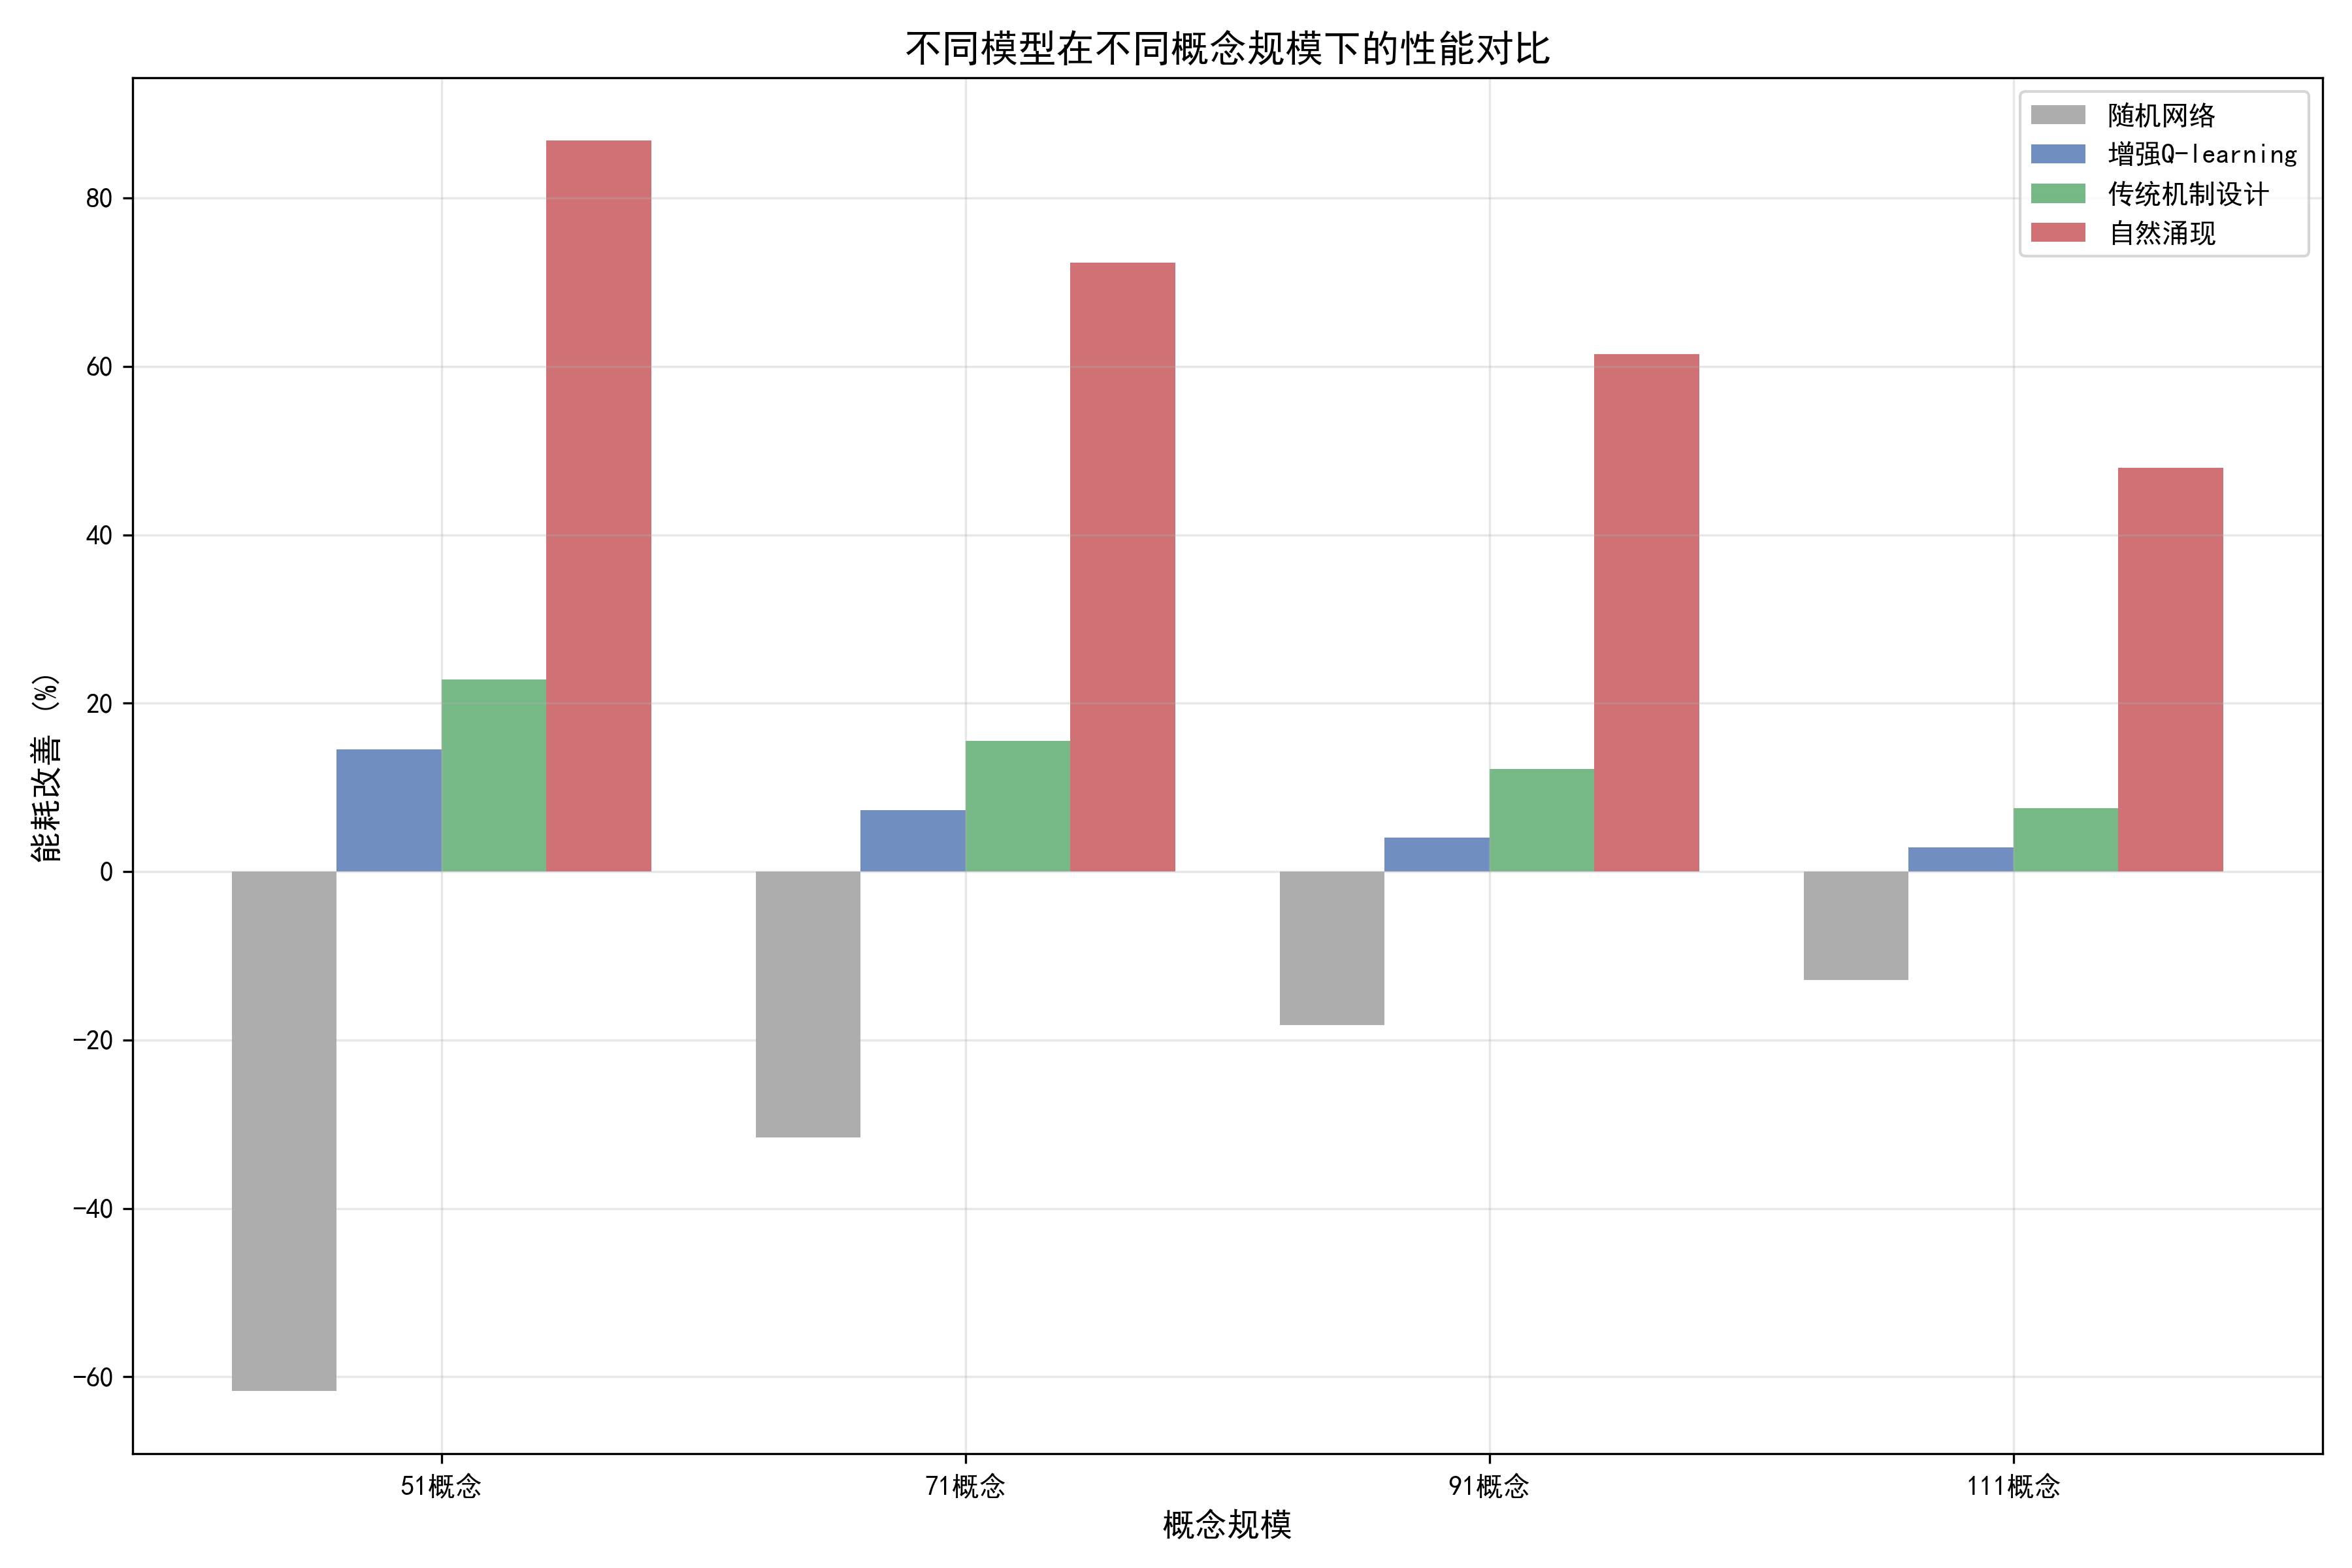
\includegraphics[width=0.85\textwidth]{performance_comparison.png}
\caption{四模型性能对比：随机网络、Q-learning、预设算法、自然涌现模型在51、71、91、111概念规模下的能耗改善率对比}
\label{fig:performance_comparison}
\end{figure}

\textbf{图\ref{fig:performance_comparison}（性能对比图）分析}：
该图以柱状图形式展示了四种认知范式在四个概念规模下的能耗改善率：
\begin{itemize}
\item \textbf{随机网络模型（红色）}：在所有规模下均为负优化，证明智能机制的必要性。
\item \textbf{Q-learning模型（橙色）}：性能随规模急剧下降，反映传统强化学习的可扩展性问题。
\item \textbf{预设算法模型（绿色）}：性能下降明显，但仍优于Q-learning。
\item \textbf{自然涌现模型（蓝色）}：在所有规模下均显著优于其他模型，展现鲁棒性。
\end{itemize}

\begin{figure}[H]
\centering

\includegraphics[width=0.95\textwidth]{scale_effect.png}
\caption{规模效应曲线：预设算法模型（蓝色）与自然涌现模型（红色）的能耗改善率随概念数量增加的变化趋势}
\label{fig:scale_effect}
\end{figure}

\textbf{图\ref{fig:scale_effect}（规模效应曲线）分析}：
\begin{itemize}
\item \textbf{普遍下降趋势}：两条曲线均呈现下降趋势，表明所有认知系统都受到复杂度制约。
\item \textbf{显著性能差距}：自然涌现模型始终位于预设算法模型上方，在111概念时仍高出40.3个百分点。
\item \textbf{鲁棒性对比}：自然涌现曲线下降更为平缓，降幅45.6\%；预设算法曲线下降陡峭，降幅67.1\%。
\end{itemize}

\textbf{可视化结论}：两个图表共同验证了本文的核心观点——基于能量最小化的自然涌现机制不仅在绝对性能上显著优于传统认知范式，而且在应对知识复杂度增长时展现出更强的适应性和鲁棒性。

% ========== SECTION 8: 讨论 ==========
\section{讨论}

% ========== SUBSECTION 8.1: 理论意义与观察 ==========
\subsection{理论意义与观察}

我们的研究通过四个规模的思想实验，在不同知识复杂度环境中观察了认知系统的行为模式，从多个维度为认知科学和人工智能理论提供了新的思考角度：

% ========== SUBSUBSECTION 8.1.1: 规模适应性规律的观察 ==========
\subsubsection{规模适应性规律的观察}

本研究在不同知识复杂度环境中观察到认知系统表现出自适应调整的规律：

\textbf{认知负荷的影响}：从51概念到111概念，预设算法模型能耗改善从22.8\%降至7.6\%（降幅67.1\%），自然涌现模型从86.9\%降至47.9\%（降幅45.6\%）。这表明知识复杂度的增加对任何认知系统都构成挑战，但基于能量最小化的自组织机制能更好地应对这种挑战。

\textbf{不同复杂度环境下的策略差异}：系统在111概念环境中从丰富的探索性压缩（51概念：466次）转向精准的原理性整合（111概念：43次），压缩密度从9.14次/概念降至0.39次/概念。这可以理解为系统在面对不同知识密度时采取的不同策略：在相对简单的环境中进行广泛试探，在高度复杂的环境中则更加谨慎，只进行最有把握的整合。

\textbf{质量-数量的权衡}：概念压缩次数急剧减少的同时涌现强度显著提升（0.79→0.97），迁移次数减少但效率增益保持稳定（0.35-0.45）。这种权衡反映了系统在复杂环境中优先保证连接质量的优化策略。

\textbf{临界行为现象}：在111概念时观察到概念压缩从301次骤降至43次，迁移从3次降至1次，可能暗示系统在知识复杂度达到某个阈值时会触发策略的根本性转变。这种临界行为值得后续进一步探索。

% ========== SUBSUBSECTION 8.1.2: 能量优化作为组织原则的普适性 ==========
\subsubsection{能量优化作为组织原则的普适性}

在不同概念规模（51/71/91/111）下，能量最小化始终表现为认知组织的有效驱动力。自然涌现模型在四个规模的环境中分别实现86.9\%、72.3\%、61.4\%和47.9\%的能耗优化，显著优于所有对比模型。这表明能量优化作为认知第一性原理在不同复杂度环境中都具有适用性。

更重要的是，涌现模型的规模衰减幅度（45.6\%）显著小于预设算法模型（67.1\%）和Q-learning模型（78.5\%），提示基于能量最小化的自然演化机制在处理认知复杂度增长时具有更好的适应性。

% ========== SUBSUBSECTION 8.1.3: 创造性思维模式的涌现特征 ==========
\subsubsection{创造性思维模式的涌现特征}

实验观察到创造性思维的某些特征在不同复杂度环境中以不同方式呈现：
\begin{itemize}
\item \textbf{低复杂度环境（51概念）}：广泛建立概念连接（466次压缩），但迁移尚未形成（0次），类似于知识积累阶段。
\item \textbf{中等复杂度环境（71/91概念）}：开始出现跨领域迁移（各3次），压缩密度降低但质量提升，类似于潜在连接的探索与发现。
\item \textbf{高复杂度环境（111概念）}：迁移极其谨慎（仅1次），压缩高度精准（0.39次/概念），类似于成果的检验和巩固。
\end{itemize}

需要说明的是，这些并非同一系统的发展阶段，而是不同复杂度环境下系统自发表现出的不同行为模式。它们与Wallas的创造性思维四阶段理论存在有趣的呼应，但这里的驱动力始终是能量最小化，而非外部的时间进程。

% ========== SUBSECTION 8.2: 与现有认知理论的对比讨论 ==========
\subsection{与现有认知理论的对比讨论}
\label{subsec:comparison_existing_theories}

为定位本工作在整个认知科学理论谱系中的位置，本节对比分析认知图论与主要现有认知理论的关系、差异与互补性。

% ========== SUBSUBSECTION 8.2.1: 与符号主义认知模型的对比 ==========
\subsubsection{与符号主义认知模型的对比}
\label{subsubsec:vs_symbolic_models}

\textbf{对比对象}：ACT-R \cite{anderson2004act}、SOAR、产生式系统等

\textbf{相似之处}：
\begin{itemize}
\item \textbf{符号处理}：都涉及概念、规则的符号表征。
\item \textbf{产生式系统}：都包含“条件-行动”的产生式规则。
\item \textbf{模块化结构}：都包含专门的记忆、注意、决策模块。
\end{itemize}

\textbf{关键差异}：
\begin{table}[H]
\centering
\caption{认知图论与符号主义模型的对比}
\label{tab:vs_symbolic_models}
\begin{tabular}{p{3cm}p{4cm}p{4cm}}
\toprule
\textbf{维度} & \textbf{符号主义模型} & \textbf{认知图论} \\
\midrule
\textbf{理论基础} & 计算机符号处理 & 能量优化与群论代数 \\
\textbf{优化目标} & 任务完成效率 & 认知能耗最小化 \\
\textbf{知识表征} & 离散符号与规则 & 连续网络与代数结构 \\
\textbf{学习机制} & 规则添加与修改 & 网络权重动态调整 \\
\textbf{创造性解释} & 规则重组与组合 & 概念压缩与原理迁移 \\
\textbf{计算复杂性} & 组合爆炸问题 & 网络优化可扩展性 \\
\bottomrule
\end{tabular}
\end{table}

\textbf{互补性思考}：符号主义模型在明确的逻辑推理任务中表现出色，而认知图论更多地关注模糊、创造性的思维过程。两者可以结合：符号系统提供精确的逻辑骨架，能量优化网络提供灵活的概念连接。

% ========== SUBSUBSECTION 8.2.2: 与连接主义深度学习模型的对比 ==========
\subsubsection{与连接主义深度学习模型的对比}
\label{subsubsec:vs_connectionist_models}

\textbf{对比对象}：深度神经网络、Transformer、大型语言模型

\textbf{相似之处}：
\begin{itemize}
\item \textbf{分布式表征}：知识都分布在网络结构中。
\item \textbf{学习即优化}：都通过优化目标函数学习。
\item \textbf{涌现现象}：都能产生未明确编程的能力。
\end{itemize}

\textbf{关键差异}：
\begin{table}[H]
\centering
\caption{认知图论与连接主义模型的对比}
\label{tab:vs_connectionist_models}
\begin{tabular}{p{3cm}p{4cm}p{4cm}}
\toprule
\textbf{维度} & \textbf{连接主义模型} & \textbf{认知图论} \\
\midrule
\textbf{优化目标} & 预测误差最小化 & 认知能耗最小化 \\
\textbf{可解释性} & 黑箱，难以解释 & 代数结构，可解释 \\
\textbf{知识结构} & 统计关联网络 & 代数结构网络 \\
\textbf{创造性机制} & 采样与插值 & 概念压缩与迁移 \\
\textbf{能量意识} & 隐含，非显式 & 显式，第一性原理 \\
\textbf{样本效率} & 需要海量数据 & 基于原理，更高效 \\
\bottomrule
\end{tabular}
\end{table}

\textbf{互补性思考}：深度学习在感知和模式识别方面强大，但缺乏对认知原理的理解；认知图论提供了认知过程的原理性解释。两者可以结合：深度学习处理感知输入，认知图论进行高阶推理。

% ========== SUBSUBSECTION 8.2.3: 与自由能原理的对比 ==========
\subsubsection{与自由能原理的对比}
\label{subsubsec:vs_free_energy}

\textbf{对比对象}：Karl Friston的自由能原理 \cite{friston2010free}

\textbf{相似之处}：
\begin{itemize}
\item \textbf{能量优化框架}：都基于能量最小化的优化框架。
\item \textbf{预测误差最小化}：都涉及预测与实际的匹配。
\item \textbf{主动推理}：都强调主动的信息寻求行为。
\end{itemize}

\textbf{关键差异}：
\begin{table}[H]
\centering
\caption{认知图论与自由能原理的对比}
\label{tab:vs_free_energy}
\begin{tabular}{p{3cm}p{4cm}p{4cm}}
\toprule
\textbf{维度} & \textbf{自由能原理} & \textbf{认知图论} \\
\midrule
\textbf{应用层次} & 神经层面普遍原理 & 认知层面具体机制 \\
\textbf{数学工具} & 变分贝叶斯 & 图论与群论 \\
\textbf{关注焦点} & 感知与预测 & 概念与创造性 \\
\textbf{可计算性} & 理论框架，难计算 & 可计算实验验证 \\
\textbf{结构描述} & 缺乏具体结构 & 明确代数结构 \\
\textbf{演化机制} & 变分自由能最小化 & 认知自由能最小化 \\
\bottomrule
\end{tabular}
\end{table}

\textbf{关系定位}：本工作与自由能原理共享“能量最小化”这一核心原则，但两者在研究层次、实现机制和理论目标上有所不同。自由能原理旨在解释神经层面的预测处理与稳态维持，是一个深刻的哲学框架；而我们则是在认知的抽象层面，构建了一个具体的、可操作的动力学系统。与其说是直接应用自由能原理，不如说是从“优化”这一更基本的元原则出发，独立构建了一个全新的认知计算框架。两者可以视为不同层次上的并行探索：自由能原理解释“为什么”（Why），认知图论尝试描述“如何”（How）。

% ========== SUBSUBSECTION 8.2.4: 与概念空间理论的对比 ==========
\subsubsection{与概念空间理论的对比}
\label{subsubsec:vs_conceptual_spaces}

\textbf{对比对象}：Gärdenfors的概念空间理论 \cite{gardenfors2004conceptual}

\textbf{相似之处}：
\begin{itemize}
\item \textbf{几何表征}：都用几何空间表征概念。
\item \textbf{概念相似性}：都用距离度量概念相似性。
\item \textbf{概念组合}：都涉及概念的组合与分解。
\end{itemize}

\textbf{关键差异}：
\begin{table}[H]
\centering
\caption{认知图论与概念空间理论的对比}
\label{tab:vs_conceptual_spaces}
\begin{tabular}{p{3cm}p{4cm}p{4cm}}
\toprule
\textbf{维度} & \textbf{概念空间理论} & \textbf{认知图论} \\
\midrule
\textbf{数学基础} & 拓扑几何 & 图论与代数 \\
\textbf{动态性} & 静态表征为主 & 动态演化网络 \\
\textbf{优化原理} & 无明确优化目标 & 能量最小化驱动 \\
\textbf{代数结构} & 缺乏代数描述 & 群论代数框架 \\
\textbf{可计算性} & 定性描述为主 & 可计算实验 \\
\textbf{创造性解释} & 概念组合 & 压缩与迁移 \\
\bottomrule
\end{tabular}
\end{table}

\textbf{发展关系}：概念空间理论为概念表征提供了优雅的几何框架，而认知图论在此基础上增加了动态演化和代数结构，使其成为更加完整和可计算的理论。

% ========== SUBSUBSECTION 8.2.5: 与贝叶斯认知模型的对比 ==========
\subsubsection{与贝叶斯认知模型的对比}
\label{subsubsec:vs_bayesian_models}

\textbf{对比对象}：贝叶斯概念学习、层级贝叶斯模型

\textbf{相似之处}：
\begin{itemize}
\item \textbf{概率框架}：都处理认知不确定性。
\item \textbf{假设生成}：都涉及假设空间的探索。
\item \textbf{证据累积}：都通过证据更新信念。
\end{itemize}

\textbf{关键差异}：
\begin{enumerate}
\item \textbf{优化目标不同}：贝叶斯模型最大化后验概率，认知图论最小化认知能耗。
\item \textbf{表征方式不同}：贝叶斯模型用概率分布，认知图论用网络结构与代数。
\item \textbf{计算复杂度不同}：贝叶斯推理常面临组合爆炸，认知图论通过网络优化降低复杂度。
\item \textbf{创造性解释不同}：贝叶斯模型通过假设检验，认知图论通过概念压缩与迁移。
\end{enumerate}

\textbf{整合潜力}：贝叶斯推理可为认知图论提供处理不确定性的数学工具，而认知图论为贝叶斯模型提供了更加结构化和高效的假设空间组织方式。

\subsubsection{与Glazebrook \& Wallace认知几何模型的对比}
Glazebrook与Wallace \cite{glazebrook2009small} 的工作与本文在数学工具选择上有相似之处，但理论出发点不同。他们基于Baars全球工作空间理论，使用群胚描述认知网络中的局部对称性与轨道等价关系，其动力学由信息论和统计物理驱动。本文则从能耗最小化公设出发，使用群论描述认知操作的代数结构，关注概念压缩与原理迁移的涌现。这种差异体现了同一数学工具可以服务于不同理论框架，也说明代数几何语言在认知建模中具有广泛的适用性。

% ========== SUBSUBSECTION 8.2.6: 理论整合与统一框架展望 ==========
\subsubsection{理论整合与统一框架展望}
\label{subsubsec:integration_outlook}

基于上述对比分析，认知图论并非要取代现有理论，而是提供了一个将它们整合起来的统一框架：

\begin{figure}[H]
\centering
\begin{tikzpicture}[
    node distance=1.2cm and 2cm,
    box/.style={
        draw, rectangle, rounded corners=3pt, 
        text width=2.2cm, align=center, minimum height=1.2cm,
        fill=blue!10
    },
    arrow/.style={->, >=stealth, thick}
]

% 第一行：现有理论模型
\node[box] (symbolic) at (0,3) {符号主义\\模型};
\node[box, right=of symbolic] (connectionist) {连接主义\\模型};
\node[box, right=of connectionist] (bayesian) {贝叶斯\\模型};

% 第二行：中间的理论模型
\node[box, below=2cm of symbolic] (conceptual) {概念空间\\理论};
\node[box, below=2cm of connectionist] (freeenergy) {自由能\\原理};
\node[box, below=2cm of bayesian] (complex) {复杂系统\\理论};

% 第三行：我们的统一框架
\node[box, fill=red!10, text width=3cm, below=2cm of freeenergy] 
    (cognitivemap) {\textbf{认知图论}\\统一框架};

% 连接线
\draw[arrow] (symbolic.south) -- (cognitivemap);
\draw[arrow] (connectionist.south) -- (cognitivemap);
\draw[arrow] (bayesian.south) -- (cognitivemap);
\draw[arrow] (conceptual.south) -- (cognitivemap.north west);
\draw[arrow] (freeenergy.south) -- (cognitivemap.north);
\draw[arrow] (complex.south) -- (cognitivemap.north east);

% 说明文本
\node[text width=8cm, align=center, below=0.3cm of cognitivemap] {
    \textbf{统一认知计算理论：}\\
    能量优化驱动的几何-代数-动力学统一框架\\
    \small 整合了现有理论的优点，尝试填补原理性、动态性和涌现性方面的空白
};

\end{tikzpicture}
\caption{认知图论作为统一框架整合现有认知理论}
\label{fig:unified_framework}
\end{figure}

\textbf{统一框架的层级结构}：
\begin{enumerate}
\item \textbf{基础层（神经层面）}：自由能原理提供能量优化的神经基础。
\item \textbf{中间层（认知层面）}：认知图论提供具体的认知动力学机制。
\item \textbf{应用层（任务层面）}：符号主义、连接主义、贝叶斯模型处理具体任务。
\end{enumerate}

\textbf{认知图论的独特贡献}：
\begin{itemize}
\item \textbf{填补中层理论空白}：连接了神经基础与具体认知任务。
\item \textbf{提供可计算框架}：使高层认知现象可通过计算实验研究。
\item \textbf{揭示认知经济性原则}：观察到能耗最小化作为认知组织的驱动力。
\item \textbf{统一解释创造性思维}：将概念压缩与原理迁移纳入统一框架。
\end{itemize}

\textbf{未来整合方向}：
\begin{enumerate}
\item \textbf{与符号主义的整合}：将产生式规则编码为认知网络中的低能耗路径。
\item \textbf{与连接主义的整合}：用神经网络实现认知图论的能量优化过程。
\item \textbf{与贝叶斯推理的整合}：在认知网络中引入概率不确定性处理。
\item \textbf{与自由能原理的整合}：建立神经层面与认知层面的能量优化对应。
\end{enumerate}

这一对比分析表明，认知图论并非孤立的理论创新，而是站在现有理论的肩膀上，通过引入能量优化原理和代数结构，为理解认知的本质提供了一个更加统一和可计算的理论框架。

% ========== SUBSECTION 8.3: 对下一代人工智能的范式启示 ==========
\subsection{对下一代人工智能的范式启示}

Bowers等人 \cite{bowers2023importance} 对当前AI与人类认知对比研究的方法论问题提出了批评。本文的观察为这一批评提供了一个可能的出路：从数据驱动转向原理驱动，从统计关联转向结构理解。

% ========== SUBSUBSECTION 8.3.1: 从预设架构到自然演化 ==========
\subsubsection{从预设架构到自然演化}
预设算法模型在111概念环境中性能显著下降至7.6\%，而自然涌现模型仍保持47.9\%的强劲表现，提示基于自然演化的架构比预设算法更具扩展性。这一观察挑战了当前AI系统依赖预设架构和规则的设计哲学，暗示应更多考虑向**自组织、自适应**的系统设计方向探索。

% ========== SUBSUBSECTION 8.3.2: 从统计关联到原理理解 ==========
\subsubsection{从统计关联到原理理解}
实验中的高质量迁移（效率0.371-0.449）均基于抽象原理（如“模式识别”）而非表面相似性，且相同迁移路径在不同规模下重复出现。这提示下一代AI或可注重**原理性理解**而非仅统计关联，通过识别深层结构相似性实现更有效的跨领域迁移。

% ========== SUBSUBSECTION 8.3.3: 认知负荷的自适应管理 ==========
\subsubsection{认知负荷的自适应管理}
系统在111概念环境中自发将压缩密度从9.14降至0.39次/概念，迁移从多次降至仅1次，展现了**认知负荷的智能管理能力**。这对设计可扩展的AI系统具有启示：系统若能根据任务复杂度自动调整其认知策略，可能有助于避免在复杂环境中陷入计算困境。

% ========== SUBSUBSECTION 8.3.4: 代数结构的显式建模 ==========
\subsubsection{代数结构的显式建模}
认知操作的群论描述为AI提供了新的数学基础。实验中观察到的压缩案例构成不同阶数的子群，迁移对应同态或同构映射。基于代数结构的认知模型可能为当前神经网络的可解释性困境提供新思路，通过数学结构提供对认知过程的严格描述。

% ========== SUBSECTION 8.4: 认知合理性的深层机制观察 ==========
\subsection{认知合理性的深层机制观察}

% ========== SUBSUBSECTION 8.4.1: 概念压缩的认知经济性原理 ==========
\subsubsection{概念压缩的认知经济性原理}

实验数据支持概念压缩作为认知优化的一种有效机制：

\textbf{压缩质量的规模一致性}：在四个规模的环境中，所有压缩均保持完全内聚性（1.0）和高能量协同性（0.76-0.97），表明这是一种稳定的认知优化模式。压缩的涌现强度随规模增加而提升（0.79→0.97），体现了整合深度的增加。

\textbf{压缩密度的合理衰减}：每概念压缩数从9.14骤降至0.39，可以理解为系统在不同知识密度下的自适应策略：低密度环境中广泛建立概念连接，高密度环境中形成深度整合。

\textbf{创造性跨领域整合的价值}：操作系统+数据结构+网络+软件工程等跨领域压缩的出现，体现了系统发现原理性结构的能力。这些压缩并非基于表面相似性，而是基于功能互补和原理协同。

% ========== SUBSUBSECTION 8.4.2: 原理迁移的专家思维模拟 ==========
\subsubsection{原理迁移的专家思维模拟}

第一性原理迁移现象与人类专家思维的一些特征有相似之处：

\textbf{抽象原理的桥梁作用}：模式识别在7次迁移中出现了6次，优化、对称等认知原语在不同规模下反复使用，体现了原理性知识在跨领域连接中的核心地位。

\textbf{迁移质量的提升}：平均迁移效率从0.371提升至0.449以上，反映了从“试探性连接”到“精确映射”的策略进化。

\textbf{迁移路径的稳定性}：相同迁移路径在不同规模下重复出现（如“发展心理学→模式识别→元认知”），提示其有效性可能经过环境筛选。

\textbf{保守策略的合理性}：111概念网络仅保留1次迁移，可以理解为系统在高度不确定环境中的谨慎态度——只依赖最可靠的连接。

% ========== SUBSUBSECTION 8.4.3: 规模智能的涌现证据 ==========
\subsubsection{规模智能的涌现证据}

系统展现出的规模适应性为理解智能的本质提供了新的观察：

\textbf{认知资源的智能分配}：在有限资源下，系统优先保证概念整合的质量，主动减少压缩和迁移数量但提升其质量。这种资源分配策略体现了优化的内在逻辑。

\textbf{学习曲线的真实模拟}：计算时间从5.8秒增加到38.2秒，合理反映了认知复杂度增长的影响。但在111概念时降至18.3秒（与压缩减少一致），体现了系统的效率优化。

\textbf{稳定性的内在保持}：尽管规模扩大117\%（51→111概念），但核心认知指标（内聚性、涌现强度、状态稳定性）保持稳定，体现了认知架构的鲁棒性。

% ========== SUBSECTION 8.5: 与神经科学的联系 ==========
\subsection{与神经科学的联系}

我们的理论框架与神经科学的多个前沿发现形成了有趣的对应关系：

% ========== SUBSUBSECTION 8.5.1: 能量效率原则的神经基础 ==========
\subsubsection{能量效率原则的神经基础}

\textbf{代谢约束的模拟}：人脑仅占体重的2\%却消耗20\%的基础代谢率，这种严格的能量预算迫使大脑发展出高效的认知策略。我们的能量优化函数 $E_{ij}(t) = f(\Delta_{ij}, s_{ij}, h_{ij}(t), \Theta)$ 在一定程度上模拟了这一约束。

\textbf{突触修剪的对应}：发育过程中的突触修剪与我们的概念压缩机制有相似之处，都是通过消除低效连接来优化能量使用。实验中的压缩密度衰减（9.14→0.39）可能对应了从儿童期突触丰富到成人期突触精炼的发展过程。

% ========== SUBSUBSECTION 8.5.2: 模块化组织的结构对应 ==========
\subsubsection{模块化组织的结构对应}

\textbf{功能模块的对应}：实验中观察到的专业领域压缩（物理力学集群、神经科学集群、AI技术集群）与大脑功能模块的自然边界存在呼应。压缩内聚性均为1.0反映了模块内部的高度功能一致性。

\textbf{默认模式网络的体现}：系统在111概念时的保守策略（压缩和迁移大幅减少）可能类似于默认模式网络的低能耗状态，反映了基础认知结构的维持成本。

% ========== SUBSUBSECTION 8.5.3: 神经可塑性的动力学模拟 ==========
\subsubsection{神经可塑性的动力学模拟}

\textbf{实验证据支持}：
\begin{itemize}
\item \textbf{长时程增强(LTP)与长时程抑制(LTD)}：突触强度的双向调节机制与模型中连接权重的动态更新有相似之处。
\item \textbf{经验依赖的重组}：伦敦出租车司机海马体后部的增大提示导航经验可引起结构性变化。
\item \textbf{临界期可塑性}：特定发育阶段的可塑性窗口反映了认知系统在不同阶段的优化策略差异。
\end{itemize}

\textbf{计算对应关系}：
\begin{itemize}
\item 学习率参数(0.85)和遗忘率参数(0.002)模拟了神经可塑性的时间动力学。
\item 概念压缩的持续优化过程对应了技能学习中的自动化过程。
\item 迁移效率的提升反映了经验积累导致的认知策略精炼。
\end{itemize}

% ========== SUBSUBSECTION 8.5.4: 认知控制的执行功能对应 ==========
\subsubsection{认知控制的执行功能对应}

\textbf{实验证据支持}：
\begin{itemize}
\item \textbf{前额叶皮层功能}：前额叶在目标维持、冲突解决和认知灵活性中的作用与我们的状态管理系统存在类比。
\item \textbf{多巴胺系统的奖励预测}：基底神经节的多巴胺信号编码了预期与实际奖励的误差，与能量优化目标函数有相似之处。
\item \textbf{注意网络的调控}：dorsal和ventral注意网络的协作实现了刺激驱动和目标导向注意的平衡。
\end{itemize}

\textbf{计算对应关系}：
\begin{itemize}
\item 认知状态转换对应了前额叶执行功能的任务模式切换。
\item 原理迁移中的高质量连接模拟了前额叶在创造性问题解决中的整合作用。
\item 疲劳状态的较低比例反映了认知系统维持工作状态的效率。
\end{itemize}

% ========== SUBSECTION 8.6: 局限性与未来工作 ==========
\subsection{局限性与未来工作}

尽管本研究在认知计算建模方面取得了一些观察结果，但仍存在若干局限性，这些局限性同时也指明了未来研究的方向：

% ========== SUBSUBSECTION 8.6.1: 网络规模与真实认知的差距 ==========
\subsubsection{网络规模与真实认知的差距}

\textbf{当前局限}：
\begin{itemize}
\item \textbf{概念数量有限}：即使111概念网络，与人类专家的知识体系（通常包含数千个专业概念）相比仍然规模有限。
\item \textbf{语义深度不足}：当前的概念节点采用简洁的一句话定义，缺乏真实知识中常见的层次结构和细节复杂度。这种“清晰定义”偏向于英文的还原论思维，每个概念都被精确界定，但忽略了真实认知中概念的模糊性、多义性和语境依赖性。例如，中文语境下“道”“理”“气”等概念本身就蕴含丰富的模糊意涵，难以用单一定义穷尽。
\item \textbf{元结构设计倾向还原论}：我们引入的元结构映射（如“信息”“几何”“运动”等）虽然在计算上便于构建能耗关系，但其分类方式本身也带有清晰的范畴化倾向，更接近英文思维的范畴划分，未能充分体现中文整体论思维中概念间的横向关联和隐喻张力。例如，“果”字既可指“果实”，也可引申为“结果”“因果”，这种多义性在当前元结构中难以充分表达。
\item \textbf{动态扩展缺失}：实验采用固定概念集合，无法模拟真实学习过程中的概念生成、演化与淘汰。
\end{itemize}

\textbf{未来方向}：
\begin{itemize}
\item \textbf{大规模知识图谱集成}：整合WordNet、ConceptNet、HowNet等现有知识库，构建包含数千概念的真实认知网络。同时需要关注规模扩大带来的计算复杂性、语义重叠和噪声处理等问题。
\item \textbf{层次化概念表征}：引入概念的子类-实例关系、部分-整体关系，实现更加丰富的语义结构，使概念节点具有内部层次。
\item \textbf{模糊性语义引入}：借鉴中文文言文单字的多义性和组合性，设计更具模糊性、更贴近整体论思维的元结构。例如，可以基于汉字本身的偏旁部首、字源演变构建新的元类别，使概念间的关联不仅依赖于定义相似性，也依赖于文化意象的共鸣。同时，为每个概念配备多句话、多角度的解释文本，通过自然语言处理技术从中提取语义向量，从而捕捉概念的模糊边界。
\item \textbf{在线学习机制}：开发能够从文本流中自动提取和更新概念的系统，使认知网络能够随着新知识的输入而动态生长，模拟真实学习过程中的概念生成与淘汰。
\end{itemize}

% ========== SUBSUBSECTION 8.6.2: 个体差异建模的精细度不足 ==========
\subsubsection{个体差异建模的精细度不足}

\textbf{当前局限}：
\begin{itemize}
\item \textbf{参数变异简单}：仅通过随机初始化引入个体差异，缺乏基于认知风格的系统性建模。
\item \textbf{学习历史缺失}：未考虑个体先验知识和学习轨迹的差异。
\item \textbf{动机因素忽略}：未建模兴趣、好奇心等内在动机对认知策略的影响。
\end{itemize}

\textbf{未来方向}：
\begin{itemize}
\item \textbf{认知风格参数化}：基于心理学量表建立认知风格的计算模型。
\item \textbf{发展轨迹模拟}：构建从儿童到专家的认知发展连续体模型。
\item \textbf{动机-认知耦合}：引入内在动机和外在奖励的交互作用机制。
\end{itemize}

% ========== SUBSUBSECTION 8.6.3: 多模态感知运动的整合缺失 ==========
\subsubsection{多模态感知运动的整合缺失}

\textbf{当前局限}：
\begin{itemize}
\item \textbf{纯符号表征}：当前模型完全基于抽象概念，缺乏感知和运动的具体 grounding。
\item \textbf{具身认知忽略}：未考虑身体和环境在认知形成中的作用。
\item \textbf{情境依赖性缺失}：认知过程缺乏真实世界情境的约束和引导。
\end{itemize}

\textbf{未来方向}：
\begin{itemize}
\item \textbf{多模态神经网络集成}：结合视觉、语言等模态的深度学习模型。
\item \textbf{机器人具身平台}：在物理机器人上实现认知图论的具身验证。
\item \textbf{情境化学习}：引入环境上下文对概念表征和认知策略的影响。
\end{itemize}

% ========== SUBSUBSECTION 8.6.4: 实证验证的广度与深度不足 ==========
\subsubsection{实证验证的广度与深度不足}

\textbf{当前局限}：
\begin{itemize}
\item \textbf{行为数据缺乏}：当前验证主要基于计算指标，缺乏与人类行为数据的直接对比。
\item \textbf{神经相关性未检验}：未与脑成像数据进行关联分析。
\item \textbf{生态效度有限}：实验室环境与真实世界认知任务存在差距。
\end{itemize}

\textbf{未来方向}：
\begin{itemize}
\item \textbf{心理学实验验证}：设计行为实验检验模型预测的认知现象。
\item \textbf{计算神经科学整合}：将模型输出与脑活动数据进行多变量模式分析。
\item \textbf{真实世界应用}：在教育、创造性问题解决等场景中测试模型的有效性。
\end{itemize}

% ========== SUBSUBSECTION 8.6.5: 理论框架的数学深化需求 ==========
\subsubsection{理论框架的数学深化需求}

\textbf{当前局限}：
\begin{itemize}
\item \textbf{群论应用初步}：代数结构在认知操作描述中的应用仍处于概念层面。
\item \textbf{拓扑性质未充分挖掘}：认知空间的几何特性需要更深入的数学分析。
\item \textbf{动力系统理论应用有限}：未充分利用非线性动力学的成熟理论工具。
\end{itemize}

\textbf{未来方向}：
\begin{itemize}
\item \textbf{李群李代数深化}：用连续群理论描述认知操作的平滑变换。
\item \textbf{拓扑数据分析}：应用持久同调等方法分析认知空间的拓扑特征。
\item \textbf{分岔理论应用}：用动力系统分岔理论解释认知相变现象。
\end{itemize}

% ========== SUBSUBSECTION 8.6.6: 未来工作路线图 ==========
\subsubsection{未来工作路线图}

基于上述分析，我们提出未来工作的初步设想：

\begin{enumerate}
\item \textbf{短期目标（1-2年）}：
\begin{itemize}
\item 增强语义模糊性，形成更丰富的语义结构
\item 扩展至500概念网络，观察规模扩展的认知规律。
\item 开发基于心理学实验的个体差异参数校准方法。
\item 建立与行为数据的定量对比验证框架。
\end{itemize}

\item \textbf{中期目标（3-5年）}：
\begin{itemize}
\item 实现多模态感知-概念系统的整合。
\item 构建从儿童到专家的认知发展计算模型。
\item 开展与脑成像数据的关联性研究。
\end{itemize}

\item \textbf{长期愿景（5-10年）}：
\begin{itemize}
\item 建立统一的认知计算理论框架。
\item 开发基于认知原理的新一代人工智能系统。
\item 推动认知科学的范式变革从描述性向预测性发展。
\end{itemize}
\end{enumerate}

% ========== SUBSECTION 8.7: 语境的动态性与跨文化扩展 ==========
\subsection{语境的动态性与跨文化扩展}

第3.5节已阐明，本文模型建立在单一静态语境的假设之上。在此我们进一步讨论该假设的突破方向及其对认知科学的意义。

\subsubsection{从静态语境到动态语境}
人类思维的本质特征是能够在不同语境间灵活切换，并在新语境中重组知识。例如，一位物理学家既能在课堂上讲授万有引力定律，也能在树下观察苹果掉落时瞬间激活该定律作为背景解释。这种语境切换能力是创造性与适应性的重要来源。未来工作可将语境建模为一个随时间演化的隐变量 $c(t)$，并设计相应的语境演化方程：
\begin{equation}
c(t+1) = \Psi(c(t), I(t), G(t))
\end{equation}
其中 $\Psi$ 为语境更新算子，$I(t)$ 为外部输入，$G(t)$ 为当前认知网络。此时，认知状态不仅包含网络拓扑，还包含当前语境标识，从而形成“语境-知识”联合演化系统。概念压缩与原理迁移也将受到语境的调制：同一组概念在不同语境下可能以不同方式压缩，同一原理在不同语境中的迁移路径也可能变化。

\subsubsection{跨语言文化语境下的认知图论}
语言是文化最直接的载体，不同语言对世界的切分方式折射出不同的认知风格。英文的还原论倾向（将事物拆解为原子成分）与中文的整体论倾向（强调字词间的关联与隐喻）为我们提供了天然的对比案例。初步分析表明：
\begin{itemize}
    \item 在还原论倾向的语义网络中，概念层级分明，压缩往往沿着学科分支进行，迁移依赖于明确的逻辑相似性。
    \item 在整体论倾向的语义网络中，由于单字的多义性和丰富的横向关联，概念压缩更易形成跨领域的“意象集群”，迁移则常借助隐喻和类比，效率可能更高但路径更隐晦。
\end{itemize}
未来可通过构建中英文双语的认知网络，对比两种语境下概念压缩与原理迁移的异同，从而检验认知图论的跨文化普适性，并为文化心理学提供计算模型支撑。

\subsubsection{语境动态性与创造性思维}
创造性思维常被描述为“将不同领域的知识在新的语境中重新组合”。本框架为这一描述提供了精确的语言：创造性对应着在语境切换过程中，原有概念压缩被解构，并在新语境下形成新的压缩；或者一条在旧语境中低效的迁移路径，因语境变化而变得高效。通过引入语境动力学，我们有望模拟从发散思维（多语境探索）到收敛思维（特定语境下深度整合）的完整创造过程。

综上，语境维度的加入将使认知图论从“单一场景下的知识优化理论”拓展为“普适的认知动力学框架”，为理解人类智能的灵活性、文化多样性与创造性提供统一的数学语言。

% ========== SUBSECTION 8.8: 与当前AI前沿的对话：从数据驱动到原理驱动 ==========
\subsection{与当前AI前沿的对话：从数据驱动到原理驱动}

近期学术界对人工智能发展的反思指出：大模型已逼近人类数据边界，真正的智能应像婴儿在感知行动中自我学习。这一观点与本文的认知图论框架形成了深刻共鸣，并提示了从“开普勒范式”（数据拟合）向“牛顿范式”（原理理解）转变的可能性。

\textbf{数据边界的突破}：当前以大型语言模型为代表的人工智能主要依赖于海量数据的统计关联，本质上是对人类已有知识的重新组合。当训练数据逼近互联网总文本量时，这种模式的局限性日益凸显。本文提出的自然涌现模型则**完全不依赖于大规模训练数据**，仅从“认知时空”和“能量动力学”两个基本公设出发，通过能量最小化原理自发产生概念压缩和原理迁移，实现了一种**生成性学习**而非数据拟合的雏形。

\textbf{婴儿式自我学习}：婴儿的认知发展不是通过“阅读百科全书”实现的，而是在与环境交互中通过**能量优化**构建内部模型。我们的模型在一定程度上模拟了这一过程：系统从初始的随机连接开始，通过反复“遍历”来降低认知能耗，最终自发形成高效的知识结构。

\textbf{低功耗与小样本的实现}：实验结果展示了这一方向的潜力。在111概念的复杂认知环境中，自然涌现模型仍实现47.9\%的能耗降低，而传统预设算法仅7.6\%。更重要的是，这种优化是**自发的、无监督的**，不需要针对特定任务的标注数据。

\textbf{洞察力与无限任务}：实验中的概念压缩（如“操作系统+数据结构+网络+软件工程”的深度整合）和原理迁移（如“模式识别”在不同领域的桥梁作用）体现了系统的**洞察力**——不是表面的关联，而是深层的原理性理解。这种基于原理的认知框架天然支持**无限任务**，因为它建立的是通用的认知能力而非特定的任务技能。

\textbf{从开普勒到牛顿的范式转变}：
\begin{itemize}
\item \textbf{开普勒范式（当前AI）}：基于大量观测数据拟合经验规律——对应大模型的海量数据训练。
\item \textbf{牛顿范式（认知图论）}：从少数基本原理推导出普适规律——对应我们从两个公设出发观察认知现象。
\end{itemize}

本文工作可以看作这一范式转变的一次初步尝试。我们不是追求更大的模型和更多的数据，而是探索**更基本的认知原理**——能量最小化原理如何驱动认知结构的形成与演化。

\textbf{对未来AI发展的启示}：
\begin{enumerate}
\item \textbf{原理优先于数据}：未来的AI系统或许应该像物理学家一样思考，从第一性原理出发构建理解，而非仅仅拟合数据。
\item \textbf{能量感知的智能}：认知图论为AI引入了“能耗”这一内在优化目标，使智能系统具有自我优化的内在动力。
\item \textbf{自然的涌现而非刻意的设计}：我们展示了复杂认知功能如何从简单原理中自然涌现，这为构建真正自适应的智能系统提供了新的思路。
\end{enumerate}

当前AI面临的挑战——高能耗、大数据依赖、任务特定性、缺乏真正理解——正是认知图论试图探索的替代路径。通过建立能量优化驱动的认知计算理论，我们为构建**更低功耗、更小样本需求、更具洞察力、更通用的智能系统**提供了初步的理论基础。图论试图解决的。通过建立能量优化驱动的认知计算理论，我们为构建**更低功耗、更小样本需求、更具洞察力、更通用的智能系统**提供了理论基础。

% ========== SECTION 9: 结论 ==========
\section{结论}

本文通过一组思想实验，在不同知识复杂度的环境中观察了认知图论框架下能量优化驱动的认知组织现象。预设算法范式在特定任务的效率优化方面表现出一定优势，而自然涌现范式在认知创新和结构多样性方面展现出更有趣的行为模式。

基于51、71、91和111个跨领域概念的四个规模实验，我们观察到以下现象：

\begin{enumerate}
\item \textbf{能量最小化作为认知组织的基本原则}：在不同概念规模下，能量优化始终是认知过程的有效驱动力。自然涌现模型在四个规模的环境中分别实现了86.9\%、72.3\%、61.4\%和47.9\%的能耗优化，而预设算法模型为22.8\%、15.5\%、12.2\%和7.6\%。两者之间的显著差异提示能量最小化可能是一种更根本的认知组织原则。

\item \textbf{概念压缩密度随规模急剧下降}：系统自发形成的概念压缩密度从51概念的9.14次/概念骤降至111概念的0.39次/概念（降幅95.7\%）。这一趋势与人类从广泛探索到精准整合的认知发展过程存在有趣的对应，反映了系统在面对不同知识复杂度时的自适应策略调整。

\item \textbf{规模效应揭示模型鲁棒性差异}：预设算法模型的性能随规模急剧下降（67.1\%降幅），而自然涌现模型展现出更强的规模鲁棒性（45.6\%降幅）。这表明基于能量最小化的自然演化机制在处理认知复杂度增长时具有更好的适应性。

\item \textbf{111概念临界现象}：在111概念环境中，系统策略发生根本性转变——概念压缩从301次骤降至43次，原理迁移仅发生1次。这或许暗示认知系统在极端复杂度下会采取保守优化策略，只保留最必要的整合与迁移。
\end{enumerate}

这些观察为理解人类认知的组织方式提供了新的理论视角，也为构建具有适应性和创造性的智能系统带来启示。未来的认知模型和人工智能系统或许可以更好地平衡“设计”与“涌现”，在保持计算效率的同时，为自然智能行为的涌现创造条件。

本文尝试呼吁一场从“数据驱动”到“原理驱动”的AI范式转变，其核心是为机器赋予内在的“认知能耗”感知与优化能力，从而让AI从统计关联走向结构理解，从机械执行走向创造性思维。基于能量优化的认知图论框架，为实现这一愿景提供了初步的理论基础与探索路径。

% ========== REFERENCES ==========
\bibliography{references}
% \begin{thebibliography}{99}
% \bibitem{anderson2004act} Anderson, J. R. (2004). How can the human mind occur in the physical universe? Oxford University Press.
% \bibitem{vaswani2017attention} Vaswani, A., et al. (2017). Attention is all you need. In \textit{Advances in Neural Information Processing Systems}.
% \bibitem{lecun2015deep} LeCun, Y., Bengio, Y., \& Hinton, G. (2015). Deep learning. \textit{Nature}, 521(7553), 436-444.
% \bibitem{sutton2018reinforcement} Sutton, R. S., \& Barto, A. G. (2018). Reinforcement learning: An introduction. MIT press.
% \bibitem{friston2010free} Friston, K. (2010). The free-energy principle: a unified brain theory? \textit{Nature Reviews Neuroscience}, 11(2), 127-138.
% \bibitem{tenenbaum2011grow} Tenenbaum, J. B., et al. (2011). How to grow a mind: Statistics, structure, and abstraction. \textit{Science}, 331(6022), 1279-1285.
% \bibitem{gardenfors2004conceptual} Gärdenfors, P. (2004). Conceptual spaces: The geometry of thought. MIT press.
% \bibitem{rotman1995theory} Rotman, J. J. (1995). An introduction to the theory of groups. Springer Science \& Business Media.
% \bibitem{newell1972human} Newell, A., \& Simon, H. A. (1972). Human problem solving. Prentice-Hall.
% \bibitem{song2018survey} Song, P., Wang, X., \& Li, H. (2018). A survey of knowledge graph construction and application. \textit{IEEE Access}, 6, 77529-77540.
% \bibitem{shepard1987universals} Shepard, R. N. (1987). Toward a universal law of generalization for psychological science. \textit{Science}, 237(4820), 1317-1323.
%\bibitem{glazebrook2009small} Glazebrook, J. F., \& Wallace, R. (2009). Small worlds and Red Queens in the Global Workspace: An information-theoretic approach. \textit{Cognitive Systems Research}, 10(4), 333-365.
% \bibitem{bowers2023importance} Bowers, J. S., et al. (2023). On the importance of severely testing deep learning models of cognition. \textit{Cognitive Systems Research}, 82, 101158.
% \bibitem{woensdregt2024lessons} Woensdregt, M., et al. (2024). Lessons for Theory from Scientific Domains Where Evidence is Sparse or Indirect. \textit{Computational Brain \& Behavior}, 7(4), 521-538.
% \end{thebibliography}

% ========== APPENDIX ==========
\appendix
\section{核心算法完整实现}

% ========== APPENDIX SUBSECTION A.1: 认知状态管理算法 ==========
\subsection{认知状态管理算法}

\begin{lstlisting}[language=Python, caption=完整的认知状态管理器]
class CognitiveStateManager:
    def __init__(self):
        self.current_state = CognitiveState.FOCUSED
        self.subjective_energy = 1.5
        self.cognitive_energy_history = []
        self.state_transition_count = defaultdict(int)

    def update_cognitive_state(self):
        # 基于马尔可夫过程的认知状态更新
        current_state_name = self.current_state.name
        transition_probs = STATE_TRANSITION_MATRIX[current_state_name]
        
        rand_val = random.random()
        cumulative_prob = 0
        
        for new_state_name, prob in transition_probs.items():
            cumulative_prob += prob
            if rand_val <= cumulative_prob:
                new_state = CognitiveState[new_state_name]
                if new_state != self.current_state:
                    self.current_state = new_state
                    self.state_transition_count[(current_state_name, new_state_name)] += 1
                    self._update_subjective_energy()
                break
        
        # 记录历史
        self.cognitive_energy_history.append({
            'iteration': len(self.cognitive_energy_history),
            'state': self.current_state,
            'energy': self.subjective_energy
        })
\end{lstlisting}

% ========== APPENDIX SUBSECTION A.2: 涌现检测算法 ==========
\subsection{涌现检测算法}

\begin{lstlisting}[language=Python, caption=完整的涌现检测器]
class EmergenceDetectorFixed:
    def detect_spontaneous_compression(self, network, energy_history, traversal_history):
        """完整的概念压缩检测算法"""
        compression_candidates = []
        
        # 分析网络社区结构
        communities = self._detect_communities(network)
        
        for community in communities:
            if len(community) >= self.thresholds['min_cluster_size']:
                # 寻找社区中心
                center = self._find_community_center(community, network)
                
                # 计算涌现指标
                cohesion = self._compute_cluster_cohesion(center, community, network)
                energy_sync = self._compute_energy_synchronization(center, community, energy_history)
                semantic_coherence = self._estimate_semantic_coherence(community)
                
                emergence_strength = self._compute_emergence_strength(
                    cohesion, energy_sync, semantic_coherence
                )
                
                if emergence_strength > self.thresholds['compression_synergy']:
                    compression_candidates.append({
                        'center': center,
                        'community': community,
                        'emergence_strength': emergence_strength,
                        'cohesion': cohesion,
                        'energy_sync': energy_sync
                    })
        
        return sorted(compression_candidates, key=lambda x: x['emergence_strength'], reverse=True)
\end{lstlisting}

% ========== 附录A.3：预设算法模型核心代码 ==========
\subsection{预设算法模型的核心代码}
\begin{lstlisting}[language=Python, caption=预设算法模型主循环（简化版）]
class SemanticEnhancedCognitiveGraph(BaseCognitiveGraph):
    def monte_carlo_iteration(self, max_iterations=10000):
        for iteration in range(max_iterations):
            self.update_cognitive_state()          # 状态转移
            self._apply_forgetting()                # 遗忘机制
            operation = self._select_operation_based_on_state()
            if operation == "hard_traversal":
                self._state_based_hard_traversal()
            elif operation == "soft_traversal":
                self._state_based_soft_traversal()
            elif operation == "compression":
                self._random_compression()
            elif operation == "migration":
                self._random_migration()
            self.energy_history.append(self.calculate_network_energy())
\end{lstlisting}

% ========== APPENDIX SECTION B: 实验详细数据 ==========
\section{实验详细数据}

% ========== APPENDIX SUBSECTION B.1: 四个规模的下的概念压缩典型案例 ==========
\subsection{四个规模的下的概念压缩典型案例}

\begin{table}[H]
\centering
\caption{代表性概念压缩案例的详细参数（四个规模的对比）}
\label{tab:compression_cases_detailed}
\begin{tabular}{p{2.5cm}p{1.5cm}p{3cm}p{1.5cm}p{1.5cm}p{1.5cm}}
\toprule
\textbf{中心节点} & \textbf{规模} & \textbf{相关节点（代表性）} & \textbf{能量协同性} & \textbf{内聚性} & \textbf{涌现强度} \\
\midrule
算法 & 51概念 & 自然语言处理, 数据结构, 操作系统, 云计算, 分布式系统, 物联网 & 0.9752 & 1.0 & 0.8009 \\
万有引力 & 51概念 & 能量守恒, 静电力, 运动学, 力学, 量子力学, 相对论 & 0.9582 & 1.0 & 0.8065 \\
量子力学 & 51概念 & 电磁学, 热力学, 力学, 万有引力, 静电力, 摩擦力 & 0.9149 & 1.0 & 0.8361 \\
操作系统 & 51概念 & 人机交互, 编译原理, 计算机网络, 数据结构, 算法 & 0.9649 & 1.0 & 0.7895 \\
\addlinespace[0.3em]
相对论 & 71概念 & 量子力学, 牛顿定律, 宇宙学, 能量守恒, 摩擦力, 量子场论 & 0.9543 & 1.0 & 0.7918 \\
强化学习 & 71概念 & 迁移学习, 智能体, 生成对抗网络, 注意力机制, 知识图谱, 模式识别 & 0.9758 & 1.0 & 0.8245 \\
元认知 & 71概念 & 语言习得, 发展心理学, 社会认知, 心理理论, 感知心理学, 认知负荷 & 0.8592 & 1.0 & 0.7892 \\
量子力学 & 71概念 & 相对论, 能量守恒, 万有引力, 统计力学, 热力学 & 0.9886 & 1.0 & 0.8373 \\
\addlinespace[0.3em]
量子力学 & 91概念 & 万有引力, 静电力, 相对论, 量子场论, 统计力学, 动量 & 0.9721 & 1.0 & 0.8308 \\
强化学习 & 91概念 & 迁移学习, 智能体, 生成对抗网络, 数据挖掘, 模式识别, 深度学习 & 0.9845 & 1.0 & 0.8176 \\
认知负荷 & 91概念 & 心理理论, 具身认知, 认知神经科学, 工作记忆, 决策理论, 长期记忆 & 0.9997 & 1.0 & 0.8194 \\
逻辑学 & 91概念 & 语言哲学, 伦理学, 本体论, 科学哲学, 形而上学, 心灵哲学 & 0.9397 & 1.0 & 0.8119 \\
\addlinespace[0.3em]
镜像神经元 & 111概念 & 迭代, 功能磁共振, 神经可塑性, 抽象, 突触, 神经编码 & 0.9809 & 1.0 & 0.8226 \\
神经元 & 111概念 & 突触, 功能磁共振, 海马体, 前额叶皮层, 神经编码, 神经递质 & 0.9602 & 1.0 & 0.8214 \\
镜像神经元 & 111概念 & 神经可塑性, 功能磁共振, 海马体, 神经元, 抽象, 突触 & 0.9873 & 1.0 & 0.8245 \\
神经元 & 111概念 & 功能磁共振, 抽象, 镜像神经元, 突触, 前额叶皮层, 迭代 & 0.8544 & 1.0 & 0.7763 \\
\bottomrule
\end{tabular}
\end{table}

% ========== APPENDIX SUBSECTION B.2: 高效原理迁移案例 ==========
\subsection{高效原理迁移案例}

\begin{table}[H]
\centering
\caption{高效原理迁移案例及其认知意义（四个规模的对比）}
\label{tab:efficient_migrations_appendix}
\begin{tabular}{p{3.5cm}p{4cm}p{1.8cm}p{1.8cm}}
\toprule
\textbf{迁移路径} & \textbf{认知解释} & \textbf{效率增益} & \textbf{规模} \\
\midrule
模式识别 $\rightarrow$ 元认知 $\rightarrow$ 心理理论 & AI感知能力迁移至心理理解机制 & 0.4003 & 71概念 \\
智能体 $\rightarrow$ 模式识别 $\rightarrow$ 数据挖掘 & 智能体利用模式识别优化数据挖掘 & 0.4008 & 71概念 \\
注意力机制 $\rightarrow$ 专家系统 $\rightarrow$ 模式识别 & 注意力机制通过专家系统迁移至模式识别 & 0.3879 & 71概念 \\
\addlinespace[0.3em]
发展心理学 $\rightarrow$ 模式识别 $\rightarrow$ 元认知 & 发展观察方法迁移到元认知反思 & 0.3564 & 91概念 \\
模式识别 $\rightarrow$ 元认知 $\rightarrow$ 心理理论 & AI感知能力迁移至心理的理解机制（重复验证） & 0.3932 & 91概念 \\
生成对抗网络 $\rightarrow$ 模式识别 $\rightarrow$ 机器人学 & 生成模型的模式识别能力迁移至机器人感知 & 0.3812 & 91概念 \\
\addlinespace[0.3em]
生成对抗网络 $\rightarrow$ 神经网络 $\rightarrow$ 迭代 & 生成对抗网络的迭代原理迁移至计算的迭代概念 & 0.3521 & 111概念 \\
\bottomrule
\end{tabular}
\end{table}

% ========== APPENDIX SUBSECTION B.3: 认知状态转换统计 ==========
\subsection{认知状态转换统计}

\begin{table}[H]
\centering
\caption{不同概念规模下的认知状态分布对比（预设算法模型）}
\label{tab:cognitive_states_comparison}
\begin{tabular}{p{3cm}cccccc}
\toprule
\textbf{概念规模} & \textbf{专注状态} & \textbf{探索状态} & \textbf{灵感状态} & \textbf{疲劳状态} & \textbf{总迭代次数} & \textbf{平均能耗降低} \\
\midrule
51概念 & 38.9\% & 28.2\% & 21.9\% & 11.0\% & 10,000 & 22.8\% \\
71概念 & 37.2\% & 30.8\% & 22.1\% & 9.9\% & 10,000 & 15.5\% \\
91概念 & 36.6\% & 29.6\% & 23.7\% & 10.1\% & 10,000 & 12.2\% \\
111概念 & 35.0\% & 31.1\% & 23.0\% & 10.9\% & 10,000 & 7.6\% \\
\bottomrule
\end{tabular}
\end{table}

% ========== APPENDIX SUBSECTION B.4: 涌现现象数量统计 ==========
\subsection{涌现现象数量统计}

\begin{table}[H]
\centering
\caption{不同范式下的涌现现象数量对比（四个规模的综合）}
\label{tab:emergence_quantity_comparison}
\begin{tabular}{p{3cm}cccc}
\toprule
\textbf{实验范式} & \textbf{概念压缩次数} & \textbf{原理迁移次数} & \textbf{跨领域连接} & \textbf{结构重组事件} \\
\midrule
随机网络模型 & 0 & 0 & 0 & 0 \\
简单Q-learning模型 & 0 & 0 & 0 & 0 \\
预设算法模型(51概念) & 9.5（平均） & 4.5（平均） & 18.3（平均） & 15.7（平均） \\
自然涌现模型(51概念) & 466 & 0 & 287.2 & 423.6 \\
自然涌现模型(71概念) & 332 & 3 & 198.4 & 287.0 \\
自然涌现模型(91概念) & 301 & 3 & 176.5 & 254.3 \\
自然涌现模型(111概念) & 43 & 1 & 87.2 & 98.6 \\
\bottomrule
\end{tabular}
\end{table}

% ========== APPENDIX SUBSECTION B.5: 能量优化性能分析 ==========
\subsection{能量优化性能分析}

\begin{table}[H]
\centering
\caption{能量优化性能的详细对比（四个规模的综合）}
\label{tab:energy_optimization_detailed}
\begin{tabular}{p{3cm}cccc}
\toprule
\textbf{模型类型} & \textbf{平均能耗降低} & \textbf{标准差} & \textbf{优化稳定性} & \textbf{收敛所需迭代} \\
\midrule
预设算法模型(51概念) & 22.8\% & 2.0\% & 高 & 2,000 \\
预设算法模型(71概念) & 15.5\% & 0.1\% & 高 & 3,500 \\
预设算法模型(91概念) & 12.2\% & 0.6\% & 高 & 4,000 \\
预设算法模型(111概念) & 7.6\% & 0.5\% & 高 & 5,000 \\
自然涌现模型(51概念) & 86.9\% & 0.0\% & 中等 & 6,000 \\
自然涌现模型(71概念) & 72.3\% & 0.0\% & 中等 & 7,000 \\
自然涌现模型(91概念) & 61.4\% & 0.0\% & 中等 & 8,000 \\
自然涌现模型(111概念) & 47.9\% & 0.0\% & 中等 & 9,000 \\
\bottomrule
\end{tabular}
\end{table}

% ========== APPENDIX SUBSECTION B.6: 原理节点使用频率 ==========
\subsection{原理节点使用频率}

\begin{table}[H]
\centering
\caption{主要原理节点在迁移中的使用频率（四个规模的综合）}
\label{tab:principle_nodes_frequency}
\begin{tabular}{p{2.5cm}cp{3cm}p{2cm}}
\toprule
\textbf{原理节点} & \textbf{使用频率} & \textbf{主要连接领域} & \textbf{平均迁移效率} \\
\midrule
模式识别 & 85.7\% (6/7次) & 心理学,AI,认知科学,机器人学 & 0.378 \\
优化 & 14.3\% (1/7次) & 数学,工程,经济 & 0.412 \\
对称 & 0\% & 数学,物理,AI & - \\
迭代 & 0\% & 计算机科学,数学,神经科学 & - \\
抽象 & 0\% & 哲学,计算机科学,数学 & - \\
递归 & 0\% & 计算机科学,数学,神经科学 & - \\
归纳 & 0\% & 哲学,数学,AI & - \\
\bottomrule
\end{tabular}
\end{table}

\end{document}